\chapter{Development of Coupled Granular-Fluid Flow Modeling Tools for Pebble Bed Solid Breeders}\label{ch:cfd-dem-modeling-development}
%%%%%%%%%%%%%%%%%%%%%%%%%%%%%%%%%%%%%%%%%%%%%%%%%%%%%%%%%%%%%%%%%%%%%%%%%%%%%%%%%%%%%%%%%%%%%%%%%%%%%%%%%%%%
%%%%%%%%%%%%%%%%%%%%%%%%%%%%%%%%%%%%%%%%%%%%%%%%%%%%%%%%%%%%%%%%%%%%%%%%%%%%%%%%%%%%%%%%%%%%%%%%%%%%%%%%%%%%
%
% new section
%
%%%%%%%%%%%%%%%%%%%%%%%%%%%%%%%%%%%%%%%%%%%%%%%%%%%%%%%%%%%%%%%%%%%%%%%%%%%%%%%%%%%%%%%%%%%%%%%%%%%%%%%%%%%%
%%%%%%%%%%%%%%%%%%%%%%%%%%%%%%%%%%%%%%%%%%%%%%%%%%%%%%%%%%%%%%%%%%%%%%%%%%%%%%%%%%%%%%%%%%%%%%%%%%%%%%%%%%%%
\section{Dynamic Coupling of Fluid-particle, Volume-averaged Modeling} \label{sec:modeling-cfd-dem}

As we saw in Fig.~\ref{fig:keff-pressure}, even when stagnant in a bed of ceramic pebbles, helium plays a large role in the overall energy transport. A more comprehensive model of the thermophysics of a packed bed would therefore be sorely incomplete without including the contribution of helium. The first modeling approach adopted treats the helium as a volume-averaged thermofluid. Note, for shorthand I will frequently refer to the volume-averaged approach simply as the computational fluid dynamics (CFD) method, this will be sufficient to distinguish the approach from the second one introduced later. This will be the first of two approaches taken to consider the influence of helium's flow on thermal transport through the packed bed. In this approach, the fluid is considered in an Eulerian, continuum sense and the pebbles remain in the discrete, Lagrangian realm. The interactions of the fluid and solid are characterized by effective relationships in each discretized cell of fluid. The technique of coupling CFD to DEM was first proposed by Tsuji\etal.\cite{Tsuji1992} in 1992. Since that time, the CFD-DEM coupling approach has grown as a tool for granular flow research. A comparison of model formulation for CFD-DEM is discussed extensively by Zhou\etal\cite{Zhou2010}.






\subsection{Incorporating Helium into the DEM Framework}\label{sec:cfdem-heat-transfer}

In the standard DEM implementation (see \cref{sec:particle-dynamics}), each pebble obeys Newton's equations of motion in response to a net force acting upon it. To include the influence of helium in the DEM formulation, we simply add a drag force term to \Cref{eq:newton-translational}. The momentum balance of our Lagrangian-tracked pebble now reads,
\begin{equation}\label{eq:cfdem-dem-momentum}
	m_i  \ddt{\vec{r}_i} = m_i\vec{g} + \vec{f}_i + \beta_i V_i \Delta \vec{u}_{if}
\end{equation}
where all but the last term is identical to \Cref{eq:newton-translational}. The components of the last term are $\Delta \vec{u}_{if} = \vec{u}_f - u_i$, which is the relative velocity between the fluid and pebble, $i$; $\beta_i$, which is the inter-phase momentum exchange coefficient; and the drag acts upon the entire pebble volume, $V_i$. A discussion on the method of determination and form of the inter-phase drag coefficient will be discussed after introducing the DEM heat transfer equation.

To similarly include the influence of the interstitial helium on the temperatures of our pebbles, we must simply add a source term to the original energy balance equation of the DEM pebble, as given in \Cref{eq:thermoFirstLaw}. The inter-phase energy exchange coefficient (using consistent syntax with the momentum equation) is actually just the standard heat transfer coefficient, $h$, for a fluid moving past a sphere in a packed bed. After adding the inter-phase energy exchange coefficient, the energy balance of the particle now reads,
\begin{equation}\label{eq:cfdem-dem-energy}
	m_iC_i \ddt{T_i} = Q_{s,i} + \sum_{j=1}^Z Q_{ij} + h_i A_i \Delta T_{if}
\end{equation}
where again we have only needed to add the last term to account for the energy deposited/removed by the passing fluid. $\Delta T_{if}$ is the temperature difference, $T_f - T_i$, and the inter-phase energy exchange coefficient, $h_i$, acts upon the pebble surface area, $A_i$.

In the development of \Cref{eq:thermoFirstLaw}, it was assumed that a `conduction' Biot number was satisfied such that a lumped-capacitance method would be valid for the discrete pebbles in our ensemble. Likewise, for \Cref{eq:cfdem-dem-energy} to be valid, we must assume that the true Biot number is also $\Bi \ll 1$. However, the lumped capacitance method is generally developed in heat transfer systems without heat generation. Furthermore, considering the low conductivity of our pebble material, it is not apparent \textit{a priori} if the lumped capacitance assumption inherent in our DEM formulation is valid. I return to explore this issue in \cref{sec:ht-jeffreson-correction}.

Assuming their validity, these simple additions to the governing equations of momentum and energy of each particle are all that are necessary to incorporate helium into the DEM computations. The computations of the inter-phase exchange coefficients, $\beta_i$ and $h_i$ are discussed next.

\subsection{Inter-phase Exchange Coefficients}

The purge gas in ceramic breeders is meant to travel at very low flow rates to maximize the absorption of tritium. Furthermore, the pebble beds will always be near the close-packed limit. As such, the particle Reynolds number for these flows is often near unity and the Kozeny-Carman equation as applicable for Stokes flow is quite sufficient. However, we will employ the full Koch-Hill-Ladd (KHL) correlations which include terms for both the Stokes flow correlation (as a function of $\phi$) in the zero Reynolds number limit and the viscous effects with a Reynolds number-dependent term. The KHL correlation is of a general form, and reduces to the Kozeny-Carman correlation in the close-packed, zero Reynolds number limits.\cite{Koch2001} The nondimensional force of the KHL correlation reads,
\begin{equation}\label{eq:khl-correlation}
	F = F_0(\phi) + F_3(\phi)\Re
\end{equation}
where the viscous term of the drag is
\begin{equation}
F_0 = \begin{cases}
	\frac{1+3(\phi/2)^{1/2} + (135/64)\phi\ln\phi + 16.14\phi}{1 + 0.681\phi - 8.48 \phi^2 + 8.16\phi^3} & \text{if $\phi < 0.4$}\\
	10.0\,\frac{\phi}{(1-\phi)^3} & \text{if $\phi > 0.4$} 
	\end{cases}
\end{equation}
and the inertial component of the drag is
\begin{equation}
	F_3 = 0.0673 + 0.212\phi + 0.0232 \frac{1}{(1-\phi)^5}
\end{equation}

The correlation from Koch-Hill-Ladd provide a nondimensional drag that must simply be re-written to fit into the pattern of our inter-phase momentum exchange coefficient. The momentum exchange coefficient follows the common form by Gidaspow\cite{gidaspow1994multiphase} (actually differing from that used here by a factor of $1-\phi$ due to definitions of pressure and buoyancy in the drag force) thus,\cite{Hoef2005,Benyahia2006}
\begin{equation}\label{eq:interphase-momentum}
	\beta_{i} = \frac{18\mu_f}{d_{p,i}^2}(1-\phi_k)\phi_k F
\end{equation}
where $\mu_f$ is the fluid viscosity and the diameter of pebble $i$ is $d_{p,i}$. The packing fraction, $\phi_k$, in this equation is the local packing fraction in the fluid cell $k$. This value will differ from the global/bulk value in near-wall regions. As a short aside, container walls have long been known to theoretically and experimentally force order to the packing regardless of shape of packing.\cite{Hunt1990,Benenati1962,Baird1958} For example, the void fraction ($\epsilon = 1-\phi$) in narrow annular containers using the correlation from Mueller, as a function of wall-distance in a cylinder is,\cite{Mueller1999}
\[
\epsilon = \epsilon_0 + (1-\epsilon_0)J_0(ar^*)e^{-br^*}
\]
where $r^*$ is the nondimensional distance from the wall; here it is defined in terms of the pebble diameter, $r^* = r/d_p$. The constants, a and b, are defined in terms of the size parameter $\alpha = D/d_p$ where $D$ is the diameter of the annular tube. First, $a$ is
\[
    a= 
\begin{cases}
    7.383 - \cfrac{2.932}{\alpha - 9.864}, & \text{if }\  \alpha \geq 13\\
    8.243 - \cfrac{12.98}{\alpha + 3.156}, & \text{if} \ 13 \geq \alpha \geq 2.61
\end{cases}
\]
then
\[
b = 0.304 - \cfrac{0.724}{\alpha}
\]
The bulk void fraction is found from the correlation:
\[
\epsilon_0 = 0.379 + \cfrac{0.078}{\alpha - 1.8}
\]

The packing fractions as a function of distance from the container wall for two example sizes, diameters of 20$d_p$ and 5$d_p$, are plotted in Fig.~\ref{fig:packingDist}. This example is meant to demonstrate the varying packing fraction in a packed bed that is described with a single `bulk' or `global' packing fraction. The size of the discretized cell relative to the pebble will dictate how much of the void fraction variation is captured in the volume-averaged equations.

\begin{figure}[htbp]
\centering
	\includegraphics[width = \singleimagewidth]{figures/annular-packing-fraction.png}
	\caption{Showing the packing fraction approach the bulk value after a few pebble diameters when the pipe is 20$d_p$ and that when the pipe is only 5$d_p$, the packing fraction at any radius is not the same as the bed average.}
	\label{fig:packingDist}
\end{figure}

The correlation we have used here is just one possible option of many that have been developed historically for estimating the pressure drop / permeability / drag force of fluid in a packed bed. A short review of other correlations, their applicable ranges of fluid parameters, and other details is given in \cref{sec:modeling-pressure-drop}. The assumptions leading to \Cref{eq:K-C-non-dim} provide justification for our implementation of the KHL correlation for our packed beds of lithium ceramics.
\FloatBarrier



The inter-phase energy transfer coefficient is calculated from the Nusselt number for the helium flow in the ensemble,
\begin{equation}\label{eq:interphase-energy}
	h_i = \frac{\Nu k_f}{d_{p,i}}
\end{equation}
where $k_f$ is the thermal conductivity of the fluid. Several correlations for determining the Nusselt number are given for reference in \cref{sec:particle-convection}. In \Cref{sec:particle-convection}, we saw many different Nusselt number correlations. For the low-Reynolds number flows of the helium purge gas, the most appropriate correlation is from Wakao\etal, given in \Cref{eq:wakao}.
% We opt for the correlation provided by Li \& Mason which is applicable to a wide range of Reynolds number flows.\cite{Li2000} Their correlation reads,
% \begin{equation}\label{eq:li-mason-correlation}
% 	\Nu = \begin{cases}
% 	2+ 0.6\epsilon^n\Re_p^{1/2}\Pr^{1/3} 										& \Re_p < 200\\
% 	2+ 0.5\epsilon^n\Re_p^{1/2}\Pr^{1/3} + 0.02 \epsilon^n \Re_p^{0.8}\Pr^{1/3} & 200 < \Re_p < 1500\\
% 	2+ 0.000045\epsilon^n\Re_p^{1/2}			 								& \Re_p > 1500
% 	\end{cases}
% \end{equation}

% The correlation was developed for small spheres of polymer pellets in relatively dilute flow for which they found the exponent of the void fraction to be fit well to experiments when $n=3$. It might be argued that a different exponent might be necessary to apply this correlation to our packed beds. In practice, however, we observe that the majority of the Nusselt numbers calculated in each cell of the helium mesh are approximately $\Nu = 2$ which is the pure-conduction limit -- regardless of the exponent. For this reason, it is safe to assume $n=3$ is valid for our packed beds at this time.

From Eqs.~\ref{eq:interphase-momentum} and~\ref{eq:interphase-energy}, we have a formulation wherein knowledge of the flow field around our pebbles will allow calculation of dimensionless drag, $F$, and Nusselt number, $\Nu$,  and thereby the two inter-phase exchange coefficients. The flow is coupled to our DEM computations with simple algebraic additions to the equations of motion and energy of the pebble.




\subsection{Volume-averaged Thermofluid Flow}

The gas phase flow field will be treated in a method analogous to the approach of volume-averaging theory (VAT).\cite{Sbutega2013,whitaker1999method,Tsuji1992} The VAT allows treatment of complex porous flows with smooth continuous equations. In VAT, we average over a discrete space to replace complex geometry with a fictitious, smooth, continuous medium in which quantities of interested are defined independently of whether specific locations in that space are, for instance, solid or gas.

In this formulation of the gas flow, we discretize the gas space with cells that are much larger than the individual particles; in the application of our CFD-DEM coupling, this meant approximately 5 to 6 particles per cell. With VAT, the particles themselves are not resolved in the fluid space but are simply introduced via closure terms.\cite{Sbutega2013,Horvat2006} A clear derivation of the governing equations of VAT can be found in Sbutega \& Catton\cite{Sbutega2013}. The momentum and energy of a fluid flow through a solid phase with volume-averaged Navier-Stokes and energy equations are applied to each cell, $k$, in the discretized fluid space,
\begin{subequations}\label{eq:cfd-equations}
\begin{align}
\pder[\epsilon_k \rho_f]{t} + \nabla\cdot(\epsilon_k \vec{u}_f \rho_f) &= 0\\
\pder[\epsilon_k \vec{u}_f]{t} + \nabla\cdot(\epsilon_k \vec{u}_f \vec{u}_f) &= -\frac{\epsilon_k}{\rho_f}\nabla P_f + \nabla\cdot\left(\nu_f\epsilon_k\nabla \vec{u}_f\right) - \frac{S_k}{\rho_f}\\
\pder[\epsilon_k T_f]{t} + \nabla\cdot(\epsilon_k \vec{u}_f T_f) &= \nabla\left(\epsilon_k\nabla T_f\right)-\frac{E_k}{\rho_fC_f}
\end{align}
\end{subequations}

The packing fraction in any fluid cell is calculated as a function of the volumes of particles residing in cell $k$. The computation of the void fraction is deceivingly important and is discussed in length in \cref{sec:lag-eul-mapping}.
% \begin{equation}
% 	\phi_k = \frac{1}{V_k}\sum_{\forall i \in k} V_{p,i}
% \end{equation}
% where the fluid void fraction is the complement of the solid packing fraction, $\epsilon = 1 - \phi$. 

Coupling the fluid phase to the particles happens with the closure terms in momentum and energy of $S_k$ and $E_k$, respectively. They are volume-weighted sums of the drag forces and energy exchanges for all particles in the discretized fluid cell,
\begin{subequations}\label{eq:cfd-sources}
\begin{align}
	S_k &= \frac{1}{V_k}\sum_{\forall i \in k} \beta_i V_i \Delta \vec{u}_{if} \label{eq:cfd-mom-source}\\
	E_k &= \frac{1}{V_k}\sum_{\forall i \in k} h_i A_i \Delta T_{if}
\end{align}
\end{subequations}
The inter-phase momentum and energy exchange coefficients act as the communicators between the particle information from the DEM solver and the fluid fields from CFD. Thus the motion and energy of the fluid field are intimately and dynamically coupled with the particle positions and energy. Computational time is preserved by only considering volume-averaged values in the fluid domain but important inter-particle forces are still calculated in the DEM space. The nature of the coupling, \textit{i.e.} how information is mapped between the two computational spaces, is discussed next.%The cross-communication between fluid and solid is accomplished with a coupling routine that is explained in detail in Refs. 11, 12.





\subsection{Lagrangian-Eulerian Mapping Calculations of Porosity}\label{sec:lag-eul-mapping}
\begin{figure}[t]
	\centering
	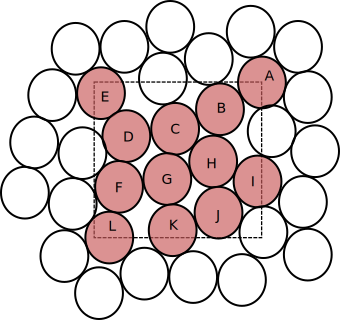
\includegraphics[width=\singleimagewidth]{figures/void-fraction-cell.pdf}
	\caption{The dashed line represents a computational cell in which exist many particles. The particles with centroids inside the cell are shaded red.}\label{fig:centroid-void-fraction}
\end{figure}
The simplest method for calculating the porosity of a CFD computational cell is to map all the DEM particles into the Eulerian volume via their centroid. We refer to this simple technique as the particle centroid method; in spite of its simplicity it is often used for large cell-to-particle volume ratios.\cite{Xu1997} A two-dimensional demonstration of the centroid technique is given in Fig.~\ref{fig:centroid-void-fraction}. In this figure, we see a computational cell (dashed line) in which many particles exist either partially or fully. The particles shaded in red have their centers located inside the cell and therefore in the simple technique have their entire volume contribute to the calculation of the porosity. The porosity for the centroid method is calculated as,
\begin{equation}
	\epsilon_\text{cell} = 1-\frac{1}{V_\text{cell}}\sum_{i = A}^{i=L}V_{p,i}
\end{equation}
where $V_{p,i}$ is the volume of particle $i$. As the cell size begins to approach the size of the particle, erroneous calculations of porosity arise. This is visible, for instance, when considering particle $A$ in Fig.~\ref{fig:centroid-void-fraction}. This particle has only a quarter of its volume inside the cell but the porosity of the cell is computed as if the entire particle existed inside. Hoomans\etal~recognized this limitation of the centroid method and introduced a fractional volume method.\cite{Hoomans1996} In the fractional volume method, the porosity is found as only partial volumes of the original sphere,
\begin{equation}
	\epsilon_\text{cell} = 1-\frac{1}{V_\text{cell}}\sum_{i = A}^{i=L}f_iV_{p,i}
\end{equation}
where $f_i$ is the fraction of the particle residing in the Eulerian cell. A similar approach taken by Kloss\etal~and Zhao \& Shan is the divided technique.\cite{Kloss2012,Zhao2013a} In this technique, the spherical particle is artificially divided into a number of regions with markers indicating their location. For example, see now how particles at the boundary, such as particle $A$, are treated in Fig.~\ref{fig:centroid-void-fraction-divided}. Instead of searching for centroids of particles, each particle has a search through the marker points (the black markers drawn in particle $A$) and the volume of that section of the sphere is assigned to whichever cell it falls inside. Note that in the sketch of Fig.~\ref{fig:centroid-void-fraction-divided}, every particle is divided with markers but particles not near the cell boundary have not had them drawn for clarity and convenience.
\begin{figure}[t]
	\centering
	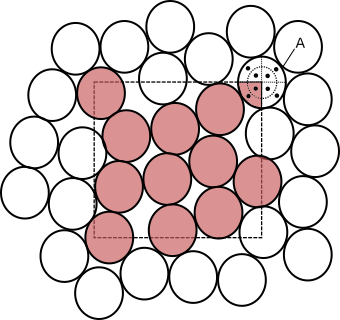
\includegraphics[width=\singleimagewidth]{figures/void-fraction-divided-cell.pdf}
	\caption{The dashed line represents a computational cell in which exist many particles. The divided portions of the particles with the sectional markers (dots) located in the cell are colored red.}\label{fig:centroid-void-fraction-divided}
\end{figure}

As the computational cell volume approaches the size of a single particle $V_\text{cell}\rightarrow V_p$, the centroid and divided techniques break down. A technique introduced by Link\etal~treats the particle as a porous cube and allows computations when a cell is completely occupied by only a single particle.\cite{Link2005} Peng\etal~offer an an analytic technique as well as guidelines for validity of either analytic or centroid techniques.\cite{Peng2014} However, in this work, I will always apply the divided technique of Kloss\etal~based on the geometry of our packed bed flow and the guidelines established by Peng\etal\cite{Kloss2012,Peng2014}


\subsection{Eulerian-Lagrangian Mapping Calculations of Force and Energy}
Once the fluid momentum and energy fields are calculated in the Eulerian grid, the coupled inter-phase exchange coefficients must map the velocities and temperatures onto the particles in the Lagrangian DEM framework. A particle centroid method is always used in the exchange onto the particles. Referencing Fig.~\ref{fig:centroid-void-fraction}, the velocity and temperature of the dashed cell is mapped only onto the particles highlighted in red. The approach has been used successfully by others.\cite{Xu1997,Link2005,Kloss2012}







\subsection{Discussion on the Applicability of CFD-DEM Governing Equations}
Early work on gas-particle flow models treated the solid and gas phases as two inter-penetrating continuum. The solid and gas were treated with the so-called two fluid model (TFM) by Anderson \& Jackson in 1967.\cite{Anderson1967} The TFM approach is similar to the VAT approach in that the fluid computational cell is sufficiently large to include many individual particles but still smaller than the size of the system.\cite{Enwald1996} The governing equations of TFM are fundamentally similar to Eqs.~\ref{eq:cfd-equations} but required constitutive equations for closure between the fluid and solid phases. Zhou\etal~show the equivalence of the governing equations of TFM and CFD-DEM.\cite{Zhou2010} The essential difference is that the issue of closure is removed with the information from DEM providing direct coupling to the fluid phase.

Since the introduction of the CFD-DEM coupling methodology by Tsuji\etal~in 1993 and then Hoomans\etal~in 1996, many researchers have adopted the approach when particle-scale information of granular and fluidized beds is important.\cite{Tsuji1993,Hoomans1996} Fluidized beds have many industrial applications and are most often studied with coupled CFD-DEM tools. A short example of work can be found in Refs.~\cite{Xu1997,Patankar2001,Swasdisevi2005,Deen2007,Zhang2008,Chu2008,VanBuijtenen2011,Gruber2012,Peng2014}

Noting the growth in application of CFD-DEM, a systematic review of the theoretical developments behind different particular system models was given by Zhu\etal\cite{Zhu2007} They consider the two most common formulations, following the notation of Gidaspow, for the governing equations. The two formulations are commonly referred to simply as Model A and Model B.\cite{gidaspow1994multiphase} Both of these models have been implemented somewhat interchangeably in CFD-DEM simulations. As pointed out by Zhu\etal, the two models differ by their treatment of the pressure drop. In Model A, the pressure drop on the system is jointly shared by the gas and solid phases. In Model B, it is only the gas phase which directly experiences the effects of pressure drop. Therefore, the two models have different forms of coupling source term, $S_k$ (see \Cref{eq:cfd-mom-source}). The source of Model B is related to that of Model A as $S_k^B = S_k^A/\epsilon - \rho_f\phi g$.

However, as is shown by Zhou\etal, there is a built-in assumption to Model B which is typically overlooked in the implementation of CFD-DEM. For an accelerating fluid, there is an added-mass in the momentum equation. In the derivation of Model B, it is tacitly assumed that the fluid is steady which is not generally valid.\cite{Zhou2010} Nevertheless, the proliferation of Model B is due to the ease in numerical implementation and, except for some situations, Model B is numerically similar to Model A for most cases studied in CFD-DEM simulations.\cite{Zhou2010} In the simulations of packed beds for tritium breeding, we choose to implement Model B as it is valid for any of the flow scenarios ever experienced by the ceramic pebble bed.







% Stability
% viscous momentum does not propagate approximately more than one cell in a single time step. If a characteristic time, $T$, is resolved with $M$ steps, then a fluid packet will travel a distance of $L$ at velocity $U$, $TU = L$. 

\subsection{Numerical Implementation of CFD-DEM}\label{sec:cfd-dem-solver}

The infrastructure for solving the DEM equations continues to be handled by LIGGGHTS. Details of the software are described in \cref{sec:dem-solver}. The DEM solver is a highly parallel C++ code based on the Molecular Dynamics (MD) code LAMMPS.\cite{Plimpton1995}

Taking advantage of a separate, stand-alone CFD solver that is maintained by a large community, the CFD simulations are conducted by the pressure-based solver using the PISO algorithm realized within the open-source framework of OpenFOAM\textsuperscript{\textregistered}.\cite{Issa1986,OpenCFDLtd2014} The coupling routines, maintained by DCS Computing GmbH, are collected in a library providing a modular framework for CFD-DEM coupling with the C++ codes LIGGGHTS and OpenFOAM\textsuperscript{\textregistered}.\cite{Kloss2012,Goniva2012}

% The helium purge gas generally flows at very small Reynolds numbers. Particle Reynolds numbers on the order of unity, $\Re\sim1$, are expected for many tritium breeding volumes. 

The routine of coupling CFD-DEM consists of several steps:
\begin{enumerate}
\item the DEM solver calculates the particles positions, velocities, and temperatures with time step dictated by stability of DEM
\item the particles positions and velocities are passed to the CFD solver using the Message Passing Interface (MPI)
\item for each particle, the cell in the CFD mesh that contains the particle is located
\item for each cell, the particle volume fraction is determined from the divided technique described in \cref{sec:lag-eul-mapping}. The ensemble-average velocity of the particles is determined
\item on the basis of $\epsilon$ and $\Re_p$, the fluid forces and heat transfer rate acting on each particle are calculated from the inter-phase exchange coefficients of Eqs.~\ref{eq:interphase-momentum} and~\ref{eq:interphase-energy}
\item the momentum and energy source/sink terms are assembled from particle-based forces by ensemble averaging over all particles in a CFD cell via Eqs.~\ref{eq:cfd-sources}
\item the inter-phase exchange coefficients of Eqs.~\ref{eq:interphase-momentum} and~\ref{eq:interphase-energy} are sent to the DEM solver
\item the CFD solver calculates the fluid velocity and temperature from the source/sink terms determined in step 6.
\item the routine is repeated from step 1
\end{enumerate}

%%%%%%%%%%%%%%%%%%%%%%%%%%%%%%%%%%%%%%%%%%%%%%%%%%%%%%%%%%%%%%%%%%%%%%%%%%%%%%%%%%%%%%%%%%%%%%%%%%%%%%%%%%%%
%%%%%%%%%%%%%%%%%%%%%%%%%%%%%%%%%%%%%%%%%%%%%%%%%%%%%%%%%%%%%%%%%%%%%%%%%%%%%%%%%%%%%%%%%%%%%%%%%%%%%%%%%%%%
%
% new section
%
%%%%%%%%%%%%%%%%%%%%%%%%%%%%%%%%%%%%%%%%%%%%%%%%%%%%%%%%%%%%%%%%%%%%%%%%%%%%%%%%%%%%%%%%%%%%%%%%%%%%%%%%%%%%
%%%%%%%%%%%%%%%%%%%%%%%%%%%%%%%%%%%%%%%%%%%%%%%%%%%%%%%%%%%%%%%%%%%%%%%%%%%%%%%%%%%%%%%%%%%%%%%%%%%%%%%%%%%%
\section{Jeffreson Correction to Lumped Capacitance Method}\label{sec:ht-jeffreson-correction}
When incorporating helium into the DEM-based modeling, the lumped capacitance assumption for each particle in the ensemble is assumed. The assumption eases the computational efforts of solving for the temperature distribution inside each particle; each particle is treated as being isothermal. The accuracy of the lumped capacitance method is described by the Biot number,
\begin{equation}
     \Bi = \frac{hd_p}{k_r}
\end{equation} 
and for $\Bi \ll 1$ the lumped capacitance method accurately models the behavior of a solid interacting with a fluid. For $\Bi \approx 0.1$ (in cases with no heat generation), the error from the lumped capacitance method is only about 5\%. In solid breeder volumes, the particles are generally small, the solid conductivity low, and heat transfer coefficient generally is also low. This leads to small-to-moderate Biot numbers expected in the packed bed. In this section we will analyze the accuracy of the lumped capacitance and introduce a correction method to account for inaccuracies of the method at moderate Biot numbers.

I simplify the case of a packed bed and only consider a single sphere with volumetric heat generation submerged in- and thermally interacting with a fluid. The sphere will be of radius $R=d_p/2$, as shown in Fig.~\ref{fig:ParticleControlVolume}. The sphere will initially be at a uniform temperature of $T_i$. The fluid temperature will remain constant at $T_f$

\begin{figure}[ht]
	\centering
		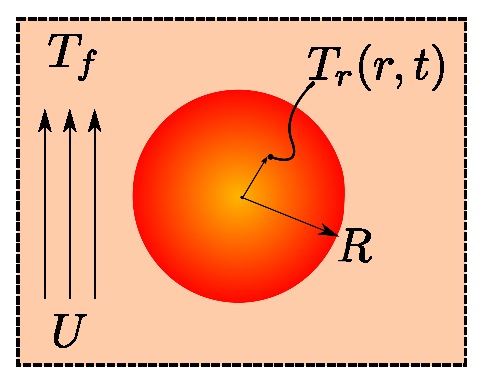
\includegraphics[width=2in]{figures/ParticleControlVolume}
	\caption[Control volume of single spherical particle in a packed bed]{Control volume of a single spherical particle in a packed bed}
	\label{fig:ParticleControlVolume}
\end{figure}


%~~~~~~~~~~~~~~~~~~~~~~~~~~~~~~~~~~~~~~~~~~~~~~~~~~~~~~~
\subsection{Lumped Capacitance Solution for Sphere}\label{sec:lumped-capacitance}
I solve for a single sphere interacting with a passing fluid, as shown in Fig.~\ref{fig:ParticleControlVolume}, while making the lumped capacitance assumption for this sphere. The solid is initially at temperature $T_0$, with constant volumetric heat generation, cooling in a fluid with constant heat transfer coefficient. The fluid will remain constant at $T_f$.

The time response of the sphere's temperature is dictated by the balance of energy to/away from the solid,  

\begin{equation}\label{eq:lc-energy-balance}
	\rho_rC_rV\frac{dT}{dt} = -hA(T-T_f) + \dot{g}V
\end{equation}

\Cref{eq:lc-energy-balance} is solved in dimensionless form with the following nondimensional parameters of temperature and time,
\begin{subequations}
\begin{align}
    \theta &= \frac{T(t) - T_f}{T_0 - T_f}\\
    \tau & = \frac{t}{R^2/\alpha}
\end{align}
\end{subequations}
where $\alpha$ is the thermal diffusivity of the sphere, $T_0$ is the initial isothermal temperature of the sphere, and $T_f$ is the constant fluid temperature. The resulting temperature distribution is,
\begin{equation}
\label{eq:theta-lc}
	\theta_{LC}=\left(1-\frac{G}{3\Bi}\right)\exp(-3\Bi \tau) + \frac{G}{3\Bi}
\end{equation}
where I have defined a dimensionless heat generation,
\begin{equation}\label{eq:nondimensional-heat-generation}
	G = \frac{\dot{g}R^2}{k(T_0 - T_f)}
\end{equation}

The energy contained in the sphere, relative to the fluid, in nondimensional terms is 
\begin{equation}
    E^*(\tau)=\frac{E(\tau)}{E_0}
\end{equation}
where $E_0$ is the initial energy of the sphere,
\begin{equation}
    E_0=\rho_rC_rV(T_0-T_f)
\end{equation}

Thus for a sphere with the lumped capacitance model, in nondimensional form, the energy is simply
\begin{equation}\label{eq:lc-energy-profile}
	E^*_{LC}(\tau) = \theta_{LC}(\tau) = \left(1-\frac{G}{3\Bi}\right)\exp(-3\Bi \tau) + \frac{G}{3\Bi}
\end{equation}

The nondimensional energy profile of \Cref{eq:lc-energy-profile} is plotted over the nondimensional time of $\tau \in [0,1/\Bi]$ in Fig.~\ref{fig:LC-sphere-in-fluid}. 

\begin{figure}[ht]
	\centering
		\includegraphics[width=\singleimagewidth]{figures/LC-sphere-in-fluid}
	\caption[Lumped Capacitance energy profile]{Lumped capacitance model: Sphere energy profile decaying from an initial value to a time of $1/\Bi$}
	\label{fig:LC-sphere-in-fluid}
\end{figure}

Reviewing \Cref{eq:theta-lc} we see that the speed of decay is dictated by the term in the exponential, $3\Bi$. Meanwhile, the steady-state value being approached is given by $\frac{G}{3\Bi} = \frac{gR}{h(T_0 - T_f)}$. It is important for this discussion to point out that because both the nondimensional heat generation and Biot number terms contain the solid conductivity, the steady-state value of the lumped capacitance model will not change for varying solid conductivity even if it leads to different Biot numbers. I will return to this point in the next section when comparing the lumped capacitance model to the exact solution when internal conduction of the solid is considered.
%~~~~~~~~~~~~~~~~~~~~~~~~~~~~~~~~~~~~~~~~~~~~~~~~~~~~~~~



%~~~~~~~~~~~~~~~~~~~~~~~~~~~~~~~~~~~~~~~~~~~~~~~~~~~~~~~
\subsection{Exact Solution for Sphere}\label{sec:analytic-sphere}

I again analyze the sphere of Fig.~\ref{fig:ParticleControlVolume} but now will account for internal temperature gradients inside the sphere. The details of the analytic solution for a sphere with heat generation interacting with a fluid is given in Appendix~\ref{sec:analytic-sphere-details}. Again, solving in terms of the nondimensional temperature and time introduced in \cref{sec:lumped-capacitance} as well as a nondimensional radius,

\begin{align*}
    \theta &= \frac{\mathbb{T}}{\mathbb{T}_0}\\
    \rho & = \frac{r}{R}\\
    \tau & = \frac{t}{R^2/\alpha}
\end{align*}

The energy conservation equation for the sphere with internal temperature gradient, in nondimensional form $\theta_{TG}$, is
\begin{equation}
    \frac{1}{\rho}\frac{\partial^2}{\partial \rho^2}(\rho\theta_{TG}) + G = \frac{\partial\theta_{TG}}{\partial \tau}
\end{equation}

With the initial condition and boundary conditions outlined in \cref{sec:analytic-sphere-details}, the nondimensional temperature distribution inside the sphere is 
\begin{equation}\label{eq:analytic-temperature-distribution}
    \theta_{TG}(\rho,\tau) = \left(\frac{G}{6} + \frac{G}{3\Bi}-\rho^2\right)  +   \sum_{n=1}^\infty \exp(-\zeta^2 \tau) \frac{\sin(\zeta_n \rho)}{\rho} \frac{Z(\zeta_n)}{N(\zeta_n)}  
\end{equation}
where $\zeta_n$ are the eigenvalues of the equation and the functions of $\zeta_n$ ($Z$,$N$,$C$) are given in \cref{sec:analytic-sphere-details}.

The accompanying nondimensional energy of the sphere is integrated to,
\begin{equation}
\label{eq:analytic-energy-profile}
    E^*_{TG}(\tau)=\left(\frac{G}{15}+\frac{G}{3\Bi}\right)+3\sum_{n=1}^\infty \exp(-\zeta^2 \tau) \frac{Z(\zeta_n)}{N(\zeta_n)} C_n(\zeta_n)
\end{equation}

I now compare the exact solution from \Cref{eq:analytic-energy-profile} to the solution of energy given by the lumped capacitance model of \Cref{eq:lc-energy-profile}. The two profiles are given in Fig.~\ref{fig:LC-analytic-sphere-in-fluid}. 

\begin{figure}[ht]
	\centering
		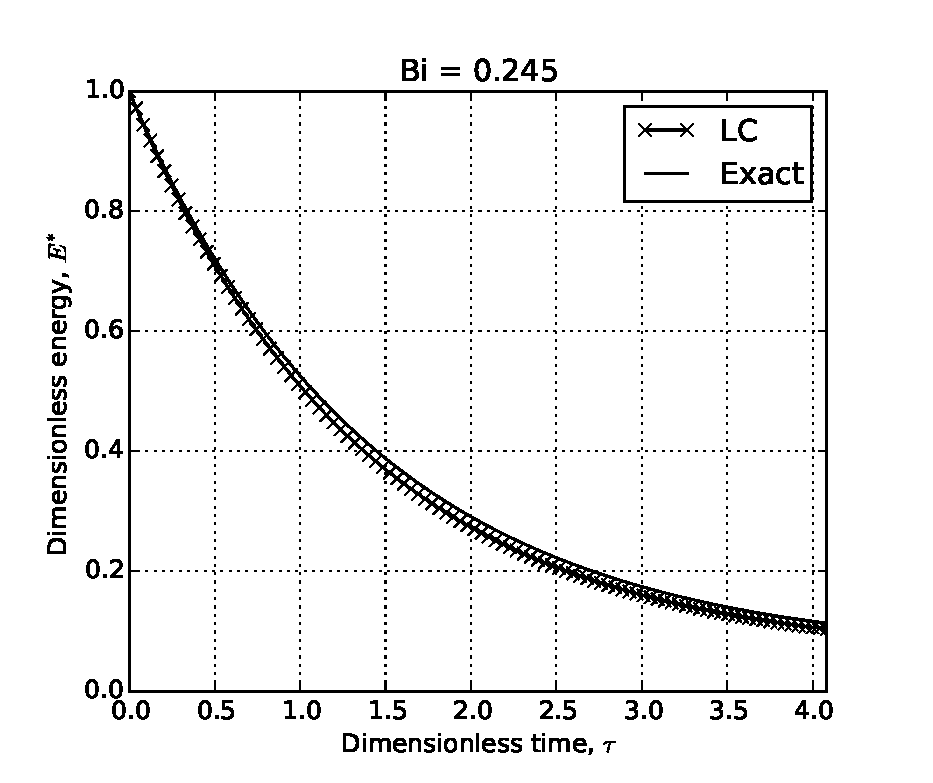
\includegraphics[width=\singleimagewidth]{figures/LC-analytic-sphere-in-fluid}
	\caption[Analytic temperature profile for $\Bi < 1$]{Analytic and lumped capacitance models: Sphere energy profile decaying from an initial value to a time of $1/\Bi$}
	\label{fig:LC-analytic-sphere-in-fluid}
\end{figure}

For the value of Biot number here, $\Bi = 0.245$, the energy profile of the analytic solution of the sphere cooling in a flow is well-captured by the lumped capacitance model. The maximum relative error over the time span, as defined by
\begin{equation}\label{eq:error}
	\text{error} = \frac{\big|E^*_{TG}(\tau) - E^*_{LC}(\tau) \big|}{E^*_{TG}(\tau)}
\end{equation}
is always less than 10\%. 

Consider now the same size sphere but with the Biot number increased by an order from: a) a conductivity of $k = k_r/10$ and b) a heat transfer coefficient of $h = 10h_f$. The two physical changes to the system result in the same Biot number ($\Bi = 2.45$) but as we can see in Fig.~\ref{fig:LC-analytic-sphere-in-fluid-Bi-2}, there are drastic differences between the energy profiles.

\begin{figure}
        \centering
        \begin{subfigure}[b]{0.5\textwidth}
                \includegraphics[width=\textwidth]{figures/LC-analytic-sphere-in-fluid-Bi-2a}
                \caption{$k \uparrow$, lumped capacitance error in the transient and steady-state.}
				\label{fig:LC-analytic-sphere-in-fluid-Bi-2a}
        \end{subfigure}%
        
          %add desired spacing between images, e. g. ~, \quad, \qquad, \hfill etc.
          %(or a blank line to force the subfigure onto a new line)
        \begin{subfigure}[b]{0.5\textwidth}
                \includegraphics[width=\textwidth]{figures/LC-analytic-sphere-in-fluid-Bi-2b}
                \caption{$h \uparrow$, lumped capacitance error mainly in the transient.}
				\label{fig:LC-analytic-sphere-in-fluid-Bi-2b}
        \end{subfigure}
        \caption[Analytic temperature profile for moderate Biot number]{Analytic and lumped capacitance models: Sphere energy profile decaying from an initial value to a time of $3/\Bi$. The same Biot number produces different results for the exact solution of a sphere with heat generation.}\label{fig:LC-analytic-sphere-in-fluid-Bi-2}
\end{figure}

Seen in Fig.~\ref{fig:LC-analytic-sphere-in-fluid-Bi-2a}, the lumped capacitance solution both over-predicts the speed at which the sphere reaches a thermal steady-state as well as the value of the steady-state. Comparatively, in Fig.~\ref{fig:LC-analytic-sphere-in-fluid-Bi-2b}, for the same Biot number, the lumped capacitance solution again over-predicts the speed to thermal steady-state by the same rate but is relatively accurate for the steady-state value itself. 

Viewing the steady-state terms of the two solutions, the source of the error becomes apparent. From \Cref{eq:analytic-energy-profile}, the steady-state term of the exact solution is
\begin{equation}
	E^*_{TG,ss}=\frac{G}{15}+\frac{G}{3\Bi}
\end{equation}

Whereas, the steady-state term of the lumped capacitance solution from \Cref{eq:lc-energy-profile} is,
\begin{equation}
	E^*_{LG,ss} = \frac{G}{3\Bi}
\end{equation}

The two steady-state values differ only by the additional term of $\frac{G}{15}$ on the exact solution. This term appears in the exact solution from integration of the temperature gradient that exists in the pebble due to volumetric heating (see \cref{sec:analytic-sphere-details}). The lumped capacitance solution assumes no internal temperature gradient in the sphere and thus by definition can not account for this $\frac{G}{15}$ term. Furthermore, the nondimensional heat generation term, $G$, given in \Cref{eq:nondimensional-heat-generation}, is importantly a function of thermal conductivity but not the heat transfer coefficient. The lack of dependence on $h$ explains the difference between steady-state values in Fig.~\ref{fig:LC-analytic-sphere-in-fluid-Bi-2}  When $\Bi$ is small, the steady state error between lumped capacitance and the exact solution is small. If only $h$ increases the error in steady-state remains small. This is demonstrated in Fig.~\ref{fig:LC-analytic-sphere-in-fluid-Bi-2b} when steady-state solutions are close. However, in Fig.~\ref{fig:LC-analytic-sphere-in-fluid-Bi-2a} as $k$ was reduced, the curves no longer converge to similar steady-states. This phenomena appears only with the combination of low conductivity materials with volumetric heating.

Even in cases without volumetric heating, when the Biot number grows large, errors appear in the transient portion of curves but ultimately converge to the same steady-state solutions. To address the inaccuracies in the time-dependent response of the lumped capacitance method with large Biot number, I make use a a correction factor such as that used by Van Lew and Xu\etal where they implemented the correction in situations without heat generation.\cite{VanLew2010,Xu2012}. In their work, they considered a heat transfer fluid interacting with a low conductivity thermal storage material. The solar thermal storage systems they analyzed often had moderate-to-large Biot numbers but they could continue to apply the lumped capacitance model in their calculations with application of a so-called Jeffreson Correction.\cite{jeffreson409} However, because their applications did not involve heat generation, I must validate its usefulness for application in our pebble beds absorbing nuclear heat.
%~~~~~~~~~~~~~~~~~~~~~~~~~~~~~~~~~~~~~~~~~~~~~~~~~~~~~~~





%~~~~~~~~~~~~~~~~~~~~~~~~~~~~~~~~~~~~~~~~~~~~~~~~~~~~~~~
\subsection{Jeffreson Correction for Sphere with Nuclear Heating}
The correlation to correct the heat transfer coefficient due to solids with large Biot number is given by Jeffreson as,\cite{jeffreson409}
\begin{equation}
	h_{p}=\frac{h}{1+\Bi/5}
\end{equation}
where $h_p$ is the modified heat transfer coefficient of the particle with an internal temperature gradient. As the Biot number increases, the modified heat transfer coefficient decreases. THe form of this correlation works to effectively slow down the rate of heat removed by the passing fluid. Recall the curves of Fig~\ref{fig:LC-analytic-sphere-in-fluid-Bi-2}. where the lumped capacitance solution over-predicted the speed with which the energy decayed towards steady-state. A modified Biot number can then also be written as
\begin{equation}\label{eq:jeffreson-correction-bip}
	\Bi_p = \frac{h_p d}{k_r} = \frac{\Bi}{1+\Bi/5}
\end{equation}

Applying the Jeffreson Correction to \Cref{eq:theta-lc}, the modified lumped capacitance solution is written now in terms of the modified Biot number,
\begin{equation}
\label{eq:theta-jc-bip}
	\theta_{JC}=\left(1-\frac{G}{3\Bi_p}\right)\exp\left(-3\Bi_p \tau\right) + \frac{G}{3\Bi_p}
\end{equation}
and thereby \Cref{eq:lc-energy-profile} also yields
\begin{equation}\label{eq:jc-energy-profile}
	E^*_{JC}(\tau) = \left(1-\frac{G}{3\Bi_p}\right)\exp\left(-3\Bi_p \tau\right) + \frac{G}{3\Bi_p}
\end{equation}

The energy profiles from the lumped capacitance model (LC), the Jeffreson correction (JC), and the exact solution are all plotted together in Fig.~\ref{fig:LC-JC-analytic-sphere-in-fluid-Bi-2}. Barely visible under the JC solution are teh curves from the exact solution. The Jeffreson correction to the lumped capacitance method allows the simple modeling approach of the lumped capacitance method to capture the proper transient as well as steady-state values for this sphere with a moderately sized Biot number. 

\begin{figure}
        \centering
        \begin{subfigure}[b]{0.5\textwidth}
                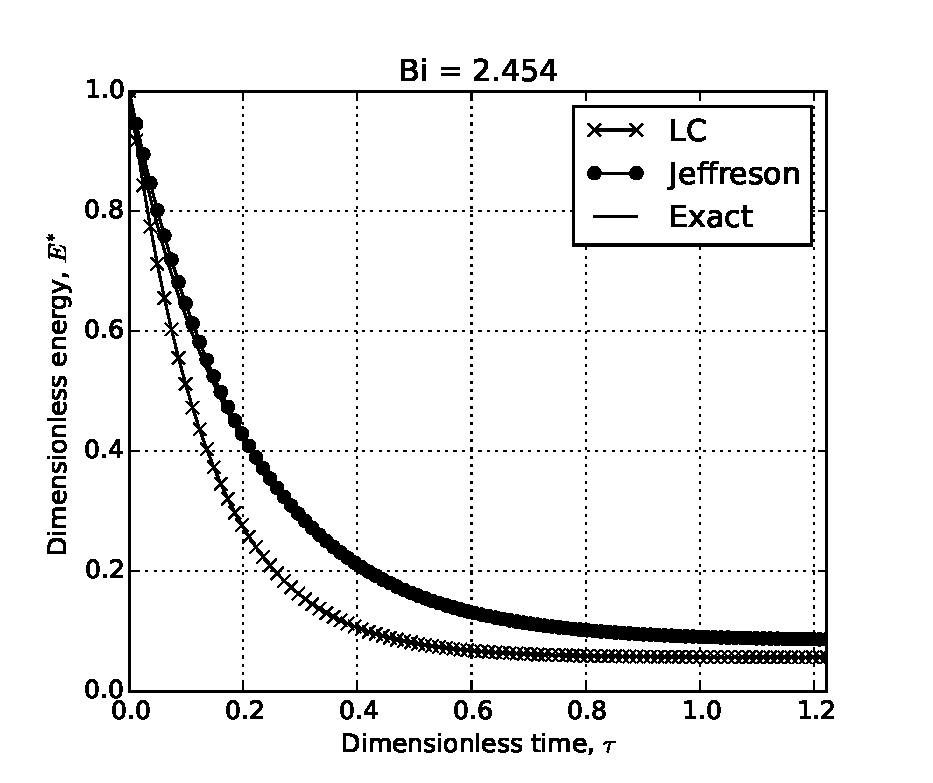
\includegraphics[width=\textwidth]{figures/LC-JC-analytic-sphere-in-fluid-Bi-2a}
                \caption{The Biot number increased from a decrease in the solid conductivity.}
				\label{fig:LC-JC-analytic-sphere-in-fluid-Bi-2a}
        \end{subfigure}%
        
          %add desired spacing between images, e. g. ~, \quad, \qquad, \hfill etc.
          %(or a blank line to force the subfigure onto a new line)
        \begin{subfigure}[b]{0.5\textwidth}
                \includegraphics[width=\textwidth]{figures/LC-JC-analytic-sphere-in-fluid-Bi-2b}
                \caption{The Biot number increased from  an increase in the heat transfer coefficient.}
				\label{fig:LC-JC-analytic-sphere-in-fluid-Bi-2b}
        \end{subfigure}
        \caption[Jeffreson correction for moderate Biot number based on conductivity]{Analytic, lumped capacitance model, and LC model with Jeffreson correction: Jeffreson correction corrects for transient and steady-state errors of lumped capacitance.}\label{fig:LC-JC-analytic-sphere-in-fluid-Bi-2}
\end{figure}

\begin{figure}
        \centering
        \begin{subfigure}[b]{0.5\textwidth}
                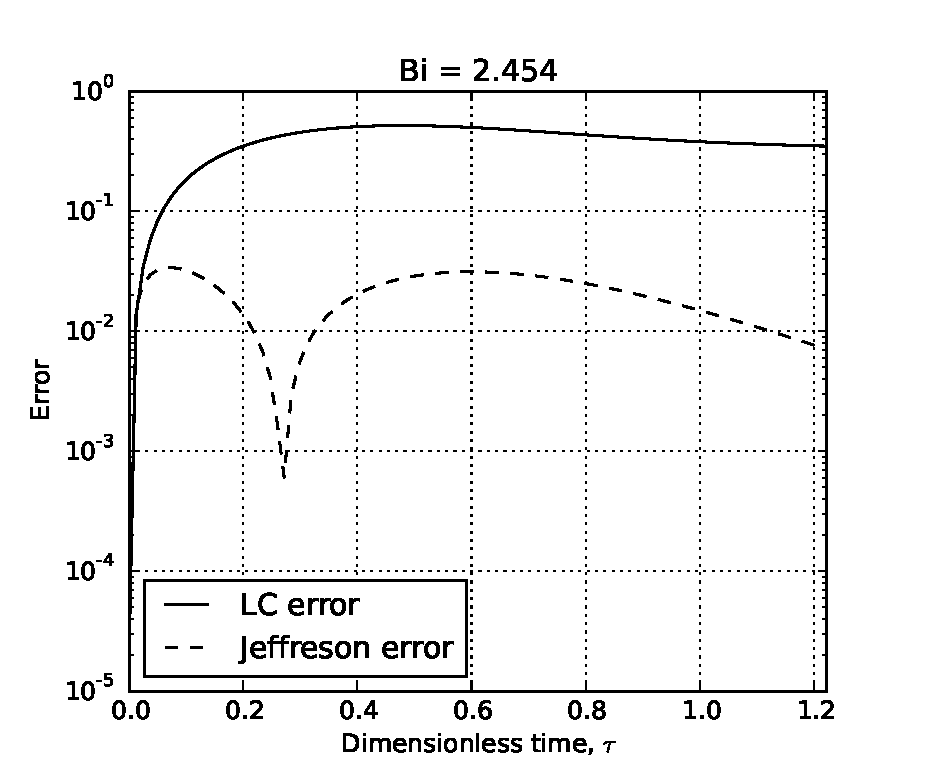
\includegraphics[width=\textwidth]{figures/LC-JC-analytic-error-Bi-2a}
                \caption{The Biot number increased from a decrease in the solid conductivity.}
				\label{fig:LC-JC-analytic-error-Bi-2a}
        \end{subfigure}%
        
          %add desired spacing between images, e. g. ~, \quad, \qquad, \hfill etc.
          %(or a blank line to force the subfigure onto a new line)
        \begin{subfigure}[b]{0.5\textwidth}
                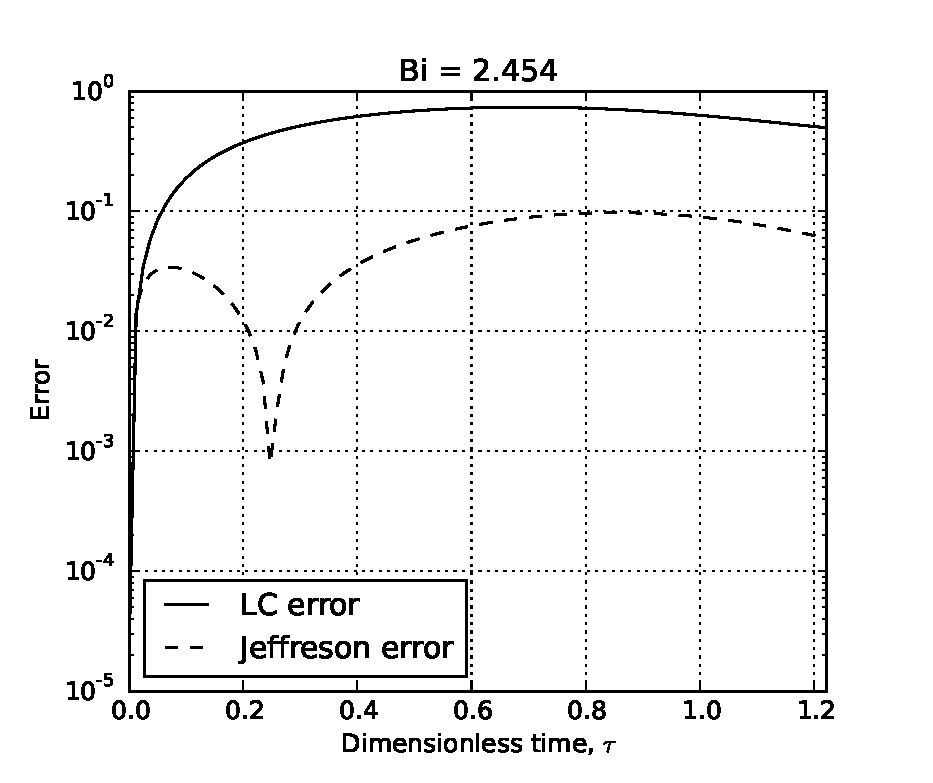
\includegraphics[width=\textwidth]{figures/LC-JC-analytic-error-Bi-2b}
                \caption{The Biot number increased from  an increase in the heat transfer coefficient.}
				\label{fig:LC-JC-analytic-error-Bi-2b}
        \end{subfigure}
        \caption[Error of lumped capacitance and Jeffreson correction for moderate Biot number]{Error of lumped capacitance and reduced error of the model with Jeffreson correction for moderate Biot number.}\label{fig:LC-JC-analytic-error-Bi-2}
\end{figure}

To look more closely, we view the instantaneous error (see \Cref{eq:error}) in Fig.~\ref{fig:LC-JC-analytic-error-Bi-2}. For the value of $\Bi > 1$ due to either low conductivity (Fig.~\ref{fig:LC-JC-analytic-error-Bi-2a}) or high heat transfer coefficient (Fig.~\ref{fig:LC-JC-analytic-error-Bi-2b}), the error in the Jeffreson correction is always under 10\%; often closer to only 1\%. This is in opposition to the standard lumped capacitance method which has 50-80\% error for both transient and steady-state values.

The lumped capacitance method allows researchers to simplify transient, conjugate heat transfer problems to a situation with an isothermal solid. In the discrete element method, the assumption of isothermal solid is innate in the framework of the method. With the implementation of the Jeffreson correction in the discrete element method, we have confidence in the fidelity of the heat transfer with the helium flow for moderately sized Biot numbers. The Jeffreson correction will be implemented into the DEM computations via \Cref{eq:jeffreson-correction-bip}. 
%~~~~~~~~~~~~~~~~~~~~~~~~~~~~~~~~~~~~~~~~~~~~~~~~~~~~~~~



%%%%%%%%%%%%%%%%%%%%%%%%%%%%%%%%%%%%%%%%%%%%%%%%%%%%%%%%%%%%%%%%%%%%%%%%%%%%%%%%%%%%%%%%%%%%%%%%%%%%%%%%%%%%
%%%%%%%%%%%%%%%%%%%%%%%%%%%%%%%%%%%%%%%%%%%%%%%%%%%%%%%%%%%%%%%%%%%%%%%%%%%%%%%%%%%%%%%%%%%%%%%%%%%%%%%%%%%%
%
% new section
%
%%%%%%%%%%%%%%%%%%%%%%%%%%%%%%%%%%%%%%%%%%%%%%%%%%%%%%%%%%%%%%%%%%%%%%%%%%%%%%%%%%%%%%%%%%%%%%%%%%%%%%%%%%%%
%%%%%%%%%%%%%%%%%%%%%%%%%%%%%%%%%%%%%%%%%%%%%%%%%%%%%%%%%%%%%%%%%%%%%%%%%%%%%%%%%%%%%%%%%%%%%%%%%%%%%%%%%%%%
\section{Summary of CFD-DEM Modeling Development}

[move this paragraph]Researchers of ceramic pebble beds for fusion reactors are concerned with damage to individual pebbles in the solid breeder volume; the accumulation of damage (\textit{e.g.} sintering, crushing) to many pebbles will ultimately have global effects on the tritium performance of the pebble bed volume.  The discrete element method provides us with the ability to probe particle-scale interactions so that we might understand, predict, and more importantly, avoid pebble damage and the morphological changes to the pebble bed associated with it. 

Simulations of heat transfer in our DEM formulation are not able to caputre the effects of an interstitial fluid. The CFD-DEM approach began as an engineering tool to study fluidized beds and as such have been benchmarked against common jet-spout fluidized beds with light-to-medium packing. However, CFD-DEM as a research tool has not before been applied to packed beds with nuclear heating such as our breeder blanket volumes. The fluid-solid heat transfer correlation, as developed for non-heat-generation situations, will continue to be employed until modifications are deemed necessary after benchmark cases are tested in the future. For now, the lumped capacitance assumption is made in the development of the heat source term for the particles in the DEM governing equations.

I tested the validity of the lumped capacitance assumption when pebbles experience heat generation with a moderately large Biot number. Seeing the inaccuracies when the solid conductivity decreased, I incorporated the Jeffreson correction to the heat transfer coefficient and showed its accuracy even under the condition of volumetric heating of the solid. The CFD-DEM approach retains pebble-scale micromechanical interaction information necessary for pebble damage modeling while computational resources are conserved with volume-averaged treatment of the flowing interstitial fluid. Closure of coupled fluid conservation equations happens with the summed contributions of particles in the fluid computation space. The correlation accounts for internal temperature gradients with negligible computational overhead.

The CFD-DEM model is a powerful and efficient means of simulating helium flow through the packed bed. However the simplicity of the volume-averaging model sacrifices the ability to resolve the complex flow fields that develop in the pebble bed. It is unclear if this simplification is completely acceptable. Therefore, concurrent to the development of the dynamic coupling of DEM to CFD, I investigated the option of a static coupling of the DEM-computed packed bed to a complete flow-solving technique.







%%%%%%%%%%%%%%%%%%%%%%%%%%%%%%%%%%%%%%%%%%%%%%%%%%%%%%%%%%%%%%%%%%%%%%%%%%%%%%%%%%%%%%%%%%%%%%%%%%%%%%%%%%%%
%%%%%%%%%%%%%%%%%%%%%%%%%%%%%%%%%%%%%%%%%%%%%%%%%%%%%%%%%%%%%%%%%%%%%%%%%%%%%%%%%%%%%%%%%%%%%%%%%%%%%%%%%%%%
%
% new section
%
%%%%%%%%%%%%%%%%%%%%%%%%%%%%%%%%%%%%%%%%%%%%%%%%%%%%%%%%%%%%%%%%%%%%%%%%%%%%%%%%%%%%%%%%%%%%%%%%%%%%%%%%%%%%
%%%%%%%%%%%%%%%%%%%%%%%%%%%%%%%%%%%%%%%%%%%%%%%%%%%%%%%%%%%%%%%%%%%%%%%%%%%%%%%%%%%%%%%%%%%%%%%%%%%%%%%%%%%%
\section{Static Coupling of Fluid-particle, Complete Modeling}\label{sec:modeling-lbm}
The volume-averaged approach of the CFD-DEM coupling is an effective and efficient method for solving transiently-coupled helium flow and pebble interaction via volume-averaging techniques for the fluid. However, there are situations when a complete knowledge of the tortuous flow of the interstitial helium may be desired. Because the CFD-DEM solver does not resolve the helium pathways on the particle scale, knowledge of precise helium flow is not possible with that scheme. Therefore a method of linking the DEM pebble beds with lattice-Boltzmann solvers is also investigated.

The lattice-Boltzmann method (LBM) to simulate fluid flow is a growing field of numerical modeling with a rich historical development. As the LBM approach is relatively new and its governing equations seem much more esoteric than the familiar conservation equations from continuum modeling, I will first go through some of the notable evolutions of the modeling history and the background physics leading to the governing equations -- which lend themselves to relatively straightforward numerical implementation. Certainly this short study cannot do justice to a proper explanation of the underlying physics. References~\cite{Chen1998a,Viggen2009,Sukop2007,Chopard2002,succi2001lattice} should be read by those curious for an excellent and thorough description of the physics, modeling approaches, and applications of LBM theory to fluid dynamics problems.




The lattice-Boltzmann is named after its mother: lattice gas automata, and its father: the Boltzmann equation from statistical mechanics. Understandably, the lattice-Boltzmann method is meant to inherit many of the advantages from both of its parents. We begin with a brief introduction to the Boltzmann equation for the statistical behavior of non-equilibrium thermodynamic systems. Then we will introduce some of the lattice gas automata predecessors to the current lattice-Boltzmann method.

\subsection{Discretized Boltzmann Equation}\label{sec:lbm-intro}

In the realm of statistical mechanics, suppose we wish to know, at a certain time $t$, how many particles exist at a given location, $\vec{x}$, that have momentum, $\vec{p}$. We define a number,
\begin{equation}
	n = f(\vec{x},\vec{p},t)\mathrm{d}\vec{x}\mathrm{d}\vec{p}
\end{equation}
as the number of $n$ particles in the system that exist within the coordinates of $\mathrm{d}\vec{x}$ and momenta $\mathrm{d}\vec{p}$ at that instant. $f(\vec{x},\vec{p},t)$ is the probability density function representing the odds of finding a particle per phase space ($\vec{x},\vec{p}$) at a moment in time, $t$.

Now let us assume we apply a small force, $\vec{F}$, to all the $n$ particles and then increment time by $\mathrm{d}t$. Assuming further that none of the particles collide (with each other or any other particles in the system), the particles will have moved an amount $\vec{x} + \frac{\vec{p}}{m}\mathrm{d}t$. The particles will all also have had their momentum changed by an amount $\vec{p} + \vec{F}\mathrm{d}t = \vec{p} + \mathrm{d}\vec{p}$. In other words, those $n$ particles are now found in the phase space of
\begin{equation}
 	n = f(\vec{x} + \frac{\vec{p}}{m}\mathrm{d}t,\vec{p} + \mathrm{d}\vec{p},t + \mathrm{d}t)\mathrm{d}\vec{x}\mathrm{d}\vec{p}
 \end{equation}

The number of particles in the two moments of time are conserved, so we can also say
\begin{equation}
	f(\vec{x} + \frac{\vec{p}}{m}\mathrm{d}t,\vec{p} + \mathrm{d}\vec{p},t + \mathrm{d}t)\mathrm{d}\vec{x}\mathrm{d}\vec{p} = f(\vec{x},\vec{p},t)\mathrm{d}\vec{x}\mathrm{d}\vec{p}
\end{equation}

Next we relax the assumption of no collisions. If we focus our attention of the phase space as before, some of the particles that began at $(\vec{x},\vec{p},t)$ will not arrive at the phase space of $(\vec{x} + \frac{\vec{p}}{m}\mathrm{d}t,\vec{p} + \mathrm{d}\vec{p},t + \mathrm{d}t)$. By the same measure, some particles that began in some other phase space \textit{will} arrive in $(\vec{x} + \frac{\vec{p}}{m}\mathrm{d}t,\vec{p} + \mathrm{d}\vec{p},t + \mathrm{d}t)$. Now the number of particles is not conserved and we write the net number of particles having left/entered this phase space as
\begin{equation}
	\Omega\mathrm{d}\vec{x}\mathrm{d}\vec{p}\mathrm{d}t
\end{equation}
where $\Omega$ is classically referred to as the collision operator. This function dictates the evolution of particles after a collision (what phase space they leave/enter). Treatment of the collision operator is itself a source for discussion but we leave it as a generic operator. Thus the balance of particles is now
\begin{equation}\label{eq:particle-balance}
	f(\vec{x} + \frac{\vec{p}}{m}\mathrm{d}t,\vec{p} + \mathrm{d}\vec{p},t + \mathrm{d}t)\mathrm{d}\vec{x}\mathrm{d}\vec{p} - f(\vec{x},\vec{p},t)\mathrm{d}\vec{x}\mathrm{d}\vec{p} = \Omega\mathrm{d}\vec{x}\mathrm{d}\vec{p}\mathrm{d}t
\end{equation}

To be precise, to arrive at the collision operator, $\Omega$, in the form we have used in \Cref{eq:particle-balance}, it is required to make a few more assumptions on the system. Following Ludwig Boltzmann, we assume: the particles are dilute, point-like, and structureless that only interact via short-range two-body potentials. Another famous assumption from Boltzmann was of \textit{Stosszahlansatz} (molecular chaos) which allow the inter-particle interactions to be described only in terms of their local binary collisions with very long paths through free space between collisions.\cite{succi2001lattice} For the sake of this discussion, we will just accept the formulation of \Cref{eq:particle-balance} as the evolution equation for the particles in our system. 

As a side note, after taking the multi-dimensional Taylor expansion of \Cref{eq:particle-balance}, we arrive at the the recognizable Boltzmann equation,
\begin{equation}\label{eq:boltzmann-continuum}
	\left[\vec{c}\cdot\nabla + \vec{F}\cdot\partial_\vec{p}  + \partial_t\right] f(\vec{x},\vec{p},t) = \Omega
\end{equation}
where $\vec{c} = \vec{p}/m$. In the form of \Cref{eq:boltzmann-continuum}, it is clear how the Boltzmann equation describes the evolution in a continuous way. There are an infinite number of directions and momenta for the particles to evolve into/from. 

However, let us discretize onto the directions of nodes in a lattice for computability. Returning to the form of \Cref{eq:particle-balance}, we normalize the mass such that $m=1$, making $\vec{p}/m = \vec{p}=\vec{c}$. Then we only allow the continuum velocity to only point in the discrete $i$ directions of neighboring nodes, $\vec{c}\rightarrow\vec{c}_i$. In discrete increments of time, we also write the collision operator in a discrete form, $\Omega\mathrm{d}t \rightarrow \Omega_i(\vec{x},t)$. Thus, \Cref{eq:particle-balance} becomes,
\begin{equation}
	f_i(\vec{x}+\vec{c}_i\Delta t, t + \Delta t) - f_i(\vec{x},t) = \Omega_i(\vec{x},t)
\end{equation}

Lastly, if we assume that we are using time units that have been normalized such that $\Delta t = 1$, the above becomes
\begin{equation}\label{eq:boltzmann2lbe}
	f_i(\vec{x}+\vec{c}_i, t + 1) - f_i(\vec{x},t) = \Omega_i(\vec{x},t)
\end{equation}

In the form of \Cref{eq:boltzmann2lbe}, our discretized version of the Boltzmann equation for statistical mechanics will be seen to be identical to a lattice-based formulation that will be arrived at purely from the point of view of the lattice gas automaton.



\subsection{Lattice Gas Automata}

In a broad sense, lattice gas automata (LGA) simulated the behavior of individual particles with a simple boolean approach where basic collision rules were defined at nodes in a lattice. As particles approached the node from neighboring nodes at a given time, the rules would dictate the direction of the particle at the next moment in time. Computationally, the particles were simply represented with boolean operators that said either 1: a particle existed at that node in that direction; or 0: no particle existed at that node in that direction. Conceptually, the particles can be thought of as hard spheres that would collide on nodes of a lattice; collisions would send the particles rebounding along discrete directions toward neighboring nodes. The restraint on collision rules required that they obey conservation of mass and momentum. 

The earliest LGA was a two-dimensional model by Hardy, Pomeau, and de Pazzis (HPP) in 1973.\cite{Hardy1975} The HPP model applied basic conservation rules that particles had to obey at each node. From the streaming particles, macroscopic units could be extracted. For instance, the particle density at a node is found from the total number of boolean particles at that node,
\begin{equation}
	\rho(\vec{x},t) = \sum_i n_i(\vec{x},t)
\end{equation}
where $n_i(\vec{x},t)$ are the particles occupying the node at $\vec{x}$ at time $t$ with a velocity of $\vec{c}_i$. As mentioned, the value of $n$ is a boolean value of 1 or 0 if the particle is present or not. Similarly, the momentum at the node is found as,
\begin{equation}
	\rho(\vec{x},t)\vec{u}(\vec{x},t) = \sum_i \vec{c}_in_i(\vec{x},t)
\end{equation}
where $\vec{u}(\vec{x},t)$ is the mean velocity of the particles at the node at that time.

The HPP model proved promising compared to other numerical methods for a number of reasons. Importantly, the boolean nature of the automata meant that the solution was not only exact (not susceptible to any round-off errors of floating point numbers) but each node required only four bits to completely describe the state (each bit described the four directions of traveling particles in the two dimensional node).\cite{Hardy1975} Furthermore, the HPP model benefited from the inherently parallel nature of all LGA simulations. The collision behavior at any given node is independent of all other nodes; the nodes only need to communicate when particles stream to neighbors.\cite{succi2001lattice}

The LGA method was given considerable more attention after 1986 when Frish, Hasslacher, and Pomeau (FHP) showed it to be possible to solve lattice gas automata simulations that were ostensibly equivalent to Navier-Stokes equations (in two dimensions).\cite{Frisch1986} Descriptions of the hexagonal lattice used in the FHP model can be found in the textbooks of Succi (Ref.~\cite{succi2001lattice}) and Sukop \& Thorne (Ref.~\cite{Sukop2007}). The FHP method gave qualitatively beautiful reproductions of hydrodynamic phenomena.

Other such LGA models were developed with the same fundamental construction as the two models mentioned here. All the models followed the same basic form of evolution of the particles. Following the form of Ref.~\cite{chopard1998cellular},
\begin{equation}\label{eq:lattice-evolution}
	n_i(\vec{x}_i + \vec{c}_i,t+1) - n_i(\vec{x},t) = \Omega_i(\vec{x},t)
\end{equation}
where, in lattices, $\Delta t = 1$ is a standard normalization. After already deriving the Boltzmann equation, \Cref{eq:lattice-evolution} is quite familiar. The equation states that the particle occupation number at a specific location and time, $n_i(\vec{x},t)$, evolves based on the collision rules, $\Omega_i(\vec{x},t)$, defined at every node, $\vec{x}$. In the LGA framework, the collision operator is much simpler than the form used in the Boltzmann equation for statistical mechanics. Here, the rules are simplified and discretized so that $\Omega_i$ can exist in a simple look-up table or explicit function of $n_i$ (with randomness).\cite{chopard1998cellular,Sukop2007}

As stated prior, the choice of collision operators is restricted only to obey conservation of mass and momentum, expressed as,
\begin{subequations}
\begin{align}
	\sum_i\Omega_i &= 0\\
	\sum_i\vec{c}_i\Omega_i&=0
\end{align}
\end{subequations}

With these simple rules applied to specific lattices, such as the LHP hexagons, it is possible to show the lattice gas automata, on a proper lattice, can be re-expressed to satisfy continuity and conservation of momentum (see Ref.~\cite{Viggen2009,Frisch1986}). The construction of LGA schemes were extremely simple yet, with their connection to conservation equations in the continuum, seemed promising as a perfect scheme for modeling fluid mechanics.

However, as exciting as the early LGA methods were, their drawbacks were very nearly as disheartening after being formally compared to the Navier-Stokes equations. Succi provides a thorough summary of the early issues with FHP (and all LGA approaches).\cite{succi2001lattice} For the sake of brevity we only mention that the main disadvantages was the lack Galilean invariance at higher Mach numbers (the results were not the same irrespective of inertial frame) and statistical noise in macroscopic quantities. The microscopic nature of LGAs -- tracking the paths of individual particles -- precluded the method from ever completely eliminating the issues such as statistical noise. The solution to the issues came in 1988 as a group zoomed-out from the microscopic into a mesoscopic formulation -- the first version of what would eventually be the lattice-Boltzmann numerical method.



\subsection{The Lattice-Boltzmann Equation}\label{sec:lbm-equations}

McNamara and Zanetti proposed a fix to the statistical noise in LGA via ensemble-averaging the boolean occupation numbers,\cite{McNamara1988}
\begin{equation}\label{eq:lbm-pdf}
	f_i = \langle n_i \rangle = \frac{1}{q}\sum_{i=1}^qn_i
\end{equation}
where $q$ is the number of lattice directions from the node. The average quantity, $f_i$, was now identical in form to the distribution function of the Boltzmann equation. In the formulation of McNamara and Zanetti, we are no longer tracking individual boolean particles but a representative ensemble population of the particles. Thus we have stepped out of the microscopic scale of individual particles into a mesoscopic realm. 

Replacing the boolean occupation numbers in \Cref{eq:lattice-evolution} with the density function of \Cref{eq:lbm-pdf}, we have
\begin{equation}\label{eq:lbm-evolution}
	f_i(\vec{x}+\vec{c}_i, t + 1) - f_i(\vec{x},t) = \Omega_i(\vec{x},t)
\end{equation}
which is precisely the form found for the discretized Boltzmann equation in \Cref{eq:boltzmann2lbe}! This is the essence of the lattice-Boltzmann method: it can be considered as a simplification of the Boltzmann concept via reduction of the continuous phase space into a finite number of discrete phase options; or it similarly can be considered as an ensemble-averaging of the lattice gas automata into calculations of mesoscopic distribution functions.

The boolean occupation numbers were simply imagined as the actual particles traveling from node to node in the LGA lattice. The ensemble average of these numbers, $f_i(\vec{x},t)$, akin to the probability density function from kinetic theory, can be envisioned to be the probability of finding a density of particles pointing in a certain direction, $i$, at a given node, $\vec{x}$, at a specific point in time, $t$. The values of $f_i$ are direction-specific fluid densities and thus macroscopic fluid properties are still directly calculated from them,
\begin{subequations}\label{eq:lbm2physical}
\begin{align}
	\rho(\vec{x},t) &= \sum_i f_i(\vec{x},t)\\
	\vec{u}(\vec{x},t) &= \frac{1}{\rho(\vec{x},t)}\sum_i \vec{c}_if_i(\vec{x},t)
\end{align}
\end{subequations}

The fluid pressure is related to the density for an ideal gas, so we can find the physical pressure in terms of the lattice density,
\begin{equation}
	p = p_0\frac{\rho(\vec{x},t)}{\rho_0}
\end{equation}

The density distribution function, while eliminating statistical noise, broke the exactness of calculations from the boolean numbers of $n_i$ in LGA methods. The density distribution function is now a floating point number, requiring more memory storage per node and introducing round-off error into calculations. In Chapter 3 of Ref.~\cite{succi2001lattice}~, Succi provides an excellent discussion of the early stages of LBM and the problems that the early models (such as those of McNamara and Zanetti) faced as well as their many great advantages. For our purposes, we accept \Cref{eq:lbm-evolution} as the fundamental equation driving the evolution of the density distribution function in a system.



\subsubsection{Collision Operator for Lattice-Boltzmann Equation}

The strength of \Cref{eq:lbm-evolution} hinges on the ability for the collision operator, $\Omega_i(\vec{x},t)$, to allow reproduction of the Navier-Stokes equations. Up to this point we have only alluded to its function in the LGA and now LBM computations. While there are many potential collision operators (see Ref.~\cite{succi2001lattice}), we focus on the operator proposed by Qian, d’Humieres, and Lallemand.\cite{qian1992lattice} Noting the similarities of LBM to kinetic theory, Qian, d'Humieres, and Lallemand proposed a collision operator similar in form to that proposed by Bhatnagar, Gross, and Krook in 1954 for the Boltzmann equation.\cite{Bhatnagar1954a} Thus the operator was named the BGK collision operator and is given as,
\begin{equation}\label{eq:bgk-operator}
	\Omega_i = -\frac{1}{\tau}\left[f_i(\vec{x},t) - f_i^\eq(\vec{x},t)\right]
\end{equation}
where $\tau$, a free parameter, is the relaxation time and $f_i^\eq$ is the equilibrium distribution. Thus in the BGK formulation, the collision operator is a relaxation of the node towards equilibrium for the density distribution function.\cite{Bhatnagar1954a}

Inserting the operator of \Cref{eq:bgk-operator} into the evolution of the density distribution function, \Cref{eq:lbm-evolution}, we have the lattice-Boltzmann evolution equation with the BGK operator,
\begin{equation}\label{eq:lbm-bgk}
	f_i(\vec{x}+\vec{c}_i, t + 1) = f_i(\vec{x},t) - \frac{1}{\tau}\left[f_i^\eq(\vec{x},t) - f_i(\vec{x},t)\right]
\end{equation}

In spite of the relaxation time being a free parameter, there are limits to its value. The kinematic viscosity in the lattice is given as,
\begin{equation}\label{eq:lbm-viscosity-relaxation-time}
	\nu = c_s^2\left(\tau-\frac{1}{2}\right)
\end{equation}
which shows that $\tau$ can not shrink to an arbitrarily small number. Numerical instabilities appear as $\tau \rightarrow 0.5$ and the kinematic viscosity $\nu \rightarrow 0$. Furthermore, if $\tau > 1$, we have subrelaxation and the distribution function will never completely relax to equilibrium. When $\tau < 1$, we have overrelaxation and the system out of equilibrium will advance toward it at different rates. When $\tau$ is small, the relaxation to $f^\eq$ is fast and thus the viscosity of the lattice can be considered to be small. A negative viscosity occurs if $\tau < 1/2$ and is not allowed.\cite{Chopard2002,Chen1998a}

The equilibrium distribution function, $f^\eq$, is derived from the Maxwell-Boltzmann velocity distribution in statistical mechanics. With clever application of the ideal gas law and the isothermal ideal gas pressure relation (see, for example, Refs.~\cite{Viggen2009,Chopard2002}), it is possible to find an equilibrium distribution that allows $\Omega_i$ to respect all conservation laws,
\begin{equation}\label{eq:equilib-dist-function}
	f_i^\eq = \rho(\vec{x},t)w_i\left[1+\frac{\vec{u}\cdot\vec{c}_i}{c_s^2} + \frac{(\vec{u}\cdot\vec{c}_i)^2}{2c_s^4} - \frac{\vec{u}^2}{2c_s^2} \right]
\end{equation}
where $c_s$ is the speed of sound on the lattice and $w_i$ are weighted lattice constants. In the development of the equilibrium function, it is assumed that the velocity of the fluid is small compared to the speed of sound on the lattice, in other words we require small Mach numbers: $\Ma = \frac{|u|}{c_s} < 1$, on the lattice.\cite{qian1992lattice,Chen1998a} It is worth noting here that the equilibrium function of \Cref{eq:equilib-dist-function} is defined entirely in terms of local velocity and density; everything is in terms of node $i$ and no other neighboring node. This feature aids the LBM approach in being highly parallelizable in the same way the LGA method was.

There are several conditions a lattice must meet to satisfy the isotropy necessary to regain the Navier-Stokes equations in the macroscopic form.\cite{Viggen2009,Latt2007} A lattice structure in $d$ dimensions with $q$ lattice directions is commonly identified with the D$d$Q$q$ lattice label. In the three-dimensional flow of our packed beds, we use the D3Q19 lattice, \textit{i.e.} $d=3$ dimensions, and $q=19$ nodes surround the node of interest (including the node itself). A representative node from the D3Q19 lattice is shown in Fig.~\ref{fig:d3q19-lattice}.
\begin{figure}[t]
	\centering
	\includegraphics[width=\singleimagewidth]{figures/lbm/4193301.jpg}
	\caption{A representative node with directional vectors to the 18 neighbors (+1 central node) in the D3Q19 lattice (reproduced from Ref.~\cite{1742-5468-2010-01-P01018}).}\label{fig:d3q19-lattice}
\end{figure}

The numbered directions in the lattice of Fig.~\ref{fig:d3q19-lattice} follows the standard practice of LBM. The index $i=0$ corresponds to the node center. The indices $i = 1,2,3,\dots,6$ point to the six faces of the cube surrounding the node. Lastly, the indices $i=7,8,9,\dots,18$ point to the twelve midpoints of the edges of the cube. The weight constants, satisfying lattice symmetry, of the lattice structure of Fig.~\ref{fig:d3q19-lattice} are calculated in Ref.~\cite{Latt2007} and given as,
\begin{equation}\label{eq:d3q19-weights}
	w_i = \begin{cases}
	\frac{1}{3}			& i = 0\\
	\frac{1}{18} 		& i = 1,2,3,\dots,6\\
	\frac{1}{36}		& i = 7,8,9,\dots,18
	\end{cases}
\end{equation}

The lattice weights, $w_i$ are necessary to account for the different vector lengths in the lattice. In principle, there is freedom in choosing the lattice speed of sound, $c_s$, requiring a change to the rest-weight of $w_0$ to maintain lattice symmetry. However, in practice, it is common to use $c_s^2 = \frac{1}{3}$ for numerical stability.\cite{Latt2007,succi2001lattice}.




\subsubsection{Boundary Conditions}
Implementation of no-slip boundary conditions at the wall in the lattice-Boltzmann method are direct descendants of the bounce-back schemes from lattice gas automata. In the scheme, lattice nodes that exist at the boundary have particle directions that point into the wall. For example, see $f_4$, $f_7$, and $f_8$ in Fig.~\ref{fig:wall-lattice-bc} for a D2Q9 lattice. The scheme is `bounce-back' because as particles stream into the wall, their distributions are scattered back in equal and opposite directions. Computationally, the bounce-back scheme is very attractive for the simplicity of implementing the method even in complex geometries. A fact which makes the use in LBM particularly attractive for packed bed simulations.\cite{Chen1998a} The bounce-back scheme has been shown to be first-order accurate for most three-dimensional flows, degrading the other-wise second order accuracy of the fluid bulk calculations.\cite{Zou1997,Chen1998a} To combat the loss in accuracy with increasing Reynolds number, several modifications to the bounce-back scheme have been proposed (see Ref.~\cite{Chen1998a}). However, for the porous flow to be studied in ceramic pebble beds, it suffices to implement the bounce-back boundary condition to enforce no-slip at the fluid-particle interface.\cite{Chen1998a,Luo2003a}

\begin{figure}[t]
	\centering
	\includegraphics[width=\singleimagewidth]{figures/lbm/ongrid}
	\caption{Sketch of the D2Q9 nodes showing at the boundary the distribution functions that would come from neighbors outside the boundary (at the wall) are unknown (drawing from correspondence with Dr. Bao, billbao@cims.nyu.edu).}\label{fig:wall-lattice-bc}
\end{figure}


To treat velocity or pressure boundary conditions, the technique of Zou \& He is used.\cite{Zou1997} They proposed extending the bounce-back condition to the non-equilibrium distribution function in the direction normal to the boundary where $\vec{v}$ or $p$ is specified. The approach allows closure of the algebraic calculation of distribution functions when we have a known velocity or pressure (see Eqs.~\ref{eq:lbm2physical}). We note again that, in lattice units, determination of density is equivalent to determination of pressure via the ideal gas pressure law. Zou \& He showed the approach provides second-order accurate results on these boundaries.\cite{Zou1997} 












\subsubsection{Thermal LBM}

Thus far the lattice-Boltzmann formulation has been shown to calculate mass and momentum transport of a fluid. But in the packed beds of fusion reactors, the transport of energy in the system is of utmost importance. To handle the thermal equations in the lattice-Boltzmann framework, we use the model of Guo\etal\cite{Guo2002} Guo\etal~introduced a second lattice upon which the distribution functions for temperature reside. The temperature distribution evolved with a coupling to the velocity distribution on the lattice solving the Navier-Stokes equations. The temperature was linked back to the Navier-Stokes lattice with a Boussinesq assumption that introduced a body force term to the fluid.\cite{Guo2002} Guo\etal~referred to their approach as the Coupled Lattice BGK (CLBGK) method. 

On the thermal lattice in the CLBGK method, the temperature is a passive scalar that is transported by the velocity (it is specified at each node corresponding to the overlapped nodes from lattice solving the Navier-Stokes equations). Therefore, the density distribution functions on the thermal lattice are actually temperature distribution functions. The thermal lattice BGK equation is analagous to \Cref{eq:lbm-bgk} and written as,
\begin{equation}\label{eq:lbm-thermal-bgk}
	g_i(\vec{x}+\vec{c}_i, t + 1) = g_i(\vec{x},t) - \frac{1}{\tau_g}\left[g_i^\eq(\vec{x},t) - g_i(\vec{x},t)\right]
\end{equation}
where we have a second relaxation time for the thermal lattice, $\tau_g$. The temperature field is reconstructed via
\begin{equation}
	T = \sum_i^q g_i
\end{equation}

A multi-scale Champan-Enskog expansion of \Cref{eq:lbm-thermal-bgk} can show that it is equivalent to the temperature form of the continuous energy conservation equation.\cite{Guo2002} For the transport of the passive scalar, we can use a D3Q7 lattice which is sufficient to model the advection-diffusion of temperature.\cite{Latt2007,Parmigiani2011}, For such a lattice, the speed of sound is $c^2_{s,g} = \frac{1}{2}$. We use a linear equilibrium function for $g_i^\eq$,
\begin{equation}
	g_i^\eq = w_i T (1+\frac{\vec{c}_i\cdot\vec{u}}{c_{s,g}^2})
\end{equation}

The thermal diffusivity (analogous to the viscosity in the momentum lattice) is 
\begin{equation}
	\alpha = c_{s,g}^2(\tau_{g} - \frac{1}{2})
\end{equation}
% The coupling from temperature to density via the Boussinesq assumption is done with the addition of a body force term, $g_i$ to the Navier-Stokes' BGK equation,
% \begin{equation}
% 	f_i^\eq = \rho(\vec{x},t)w_i\left[1+\frac{\vec{u}\cdot\vec{c}_i}{c_s^2} + \frac{(\vec{u}\cdot\vec{c}_i)^2}{2c_s^4} - \frac{\vec{u}^2}{2c_s^2} \right] + g_i
% \end{equation}
% where the body term is
% \begin{equation}
% 	g_i = -\frac{1}{2}\Delta t \alpha_i \vec{c}_i\cdot\vec{g}(T - T_0)
% \end{equation}

Thermal boundary conditions are handled via a decomposition of the boundary nodes into equilibrium and non-equilibrium parts and the values of the node extrapolated from neighboring nodes. Details of the precise equations can be found in the paper by Guo\etal.\cite{Guo2002}


\subsection{Realizing LBM Models Computationally}
Because of the immensely simple implementation of no-slip boundary conditions for even the most complex geometry, the lattice-Boltzmann method was immediately seen as a powerful option of fluid modeling in porous networks. Chen \& Doolen review many of the major accomplishments of implementing LBM models which verified Darcy's Law, the Cozeny-Karman equation, and Brinkmann equation, among other efforts.\cite{Chen1998a} Pan\etal~evaluated the single-relaxation time BGK operator against models with multiple relaxation times as well as models with different implementationsi of fluid-solid interface boundary conditions -- among which was the bounce-back scheme we use here.\cite{Pan2006}

Here we will go through the practical application of the LBM approach as it will be used  to simulate the conjugate heat transfer of the helium purge gas through ceramic pebble beds. To summarize the method, there are two main objects required to define the structure of a lattice-Boltzmann model: a collision operator, $\Omega_i$, and the constants which define the scaffolding of the lattice.

The computational domain of the fluid is discretized into a Cartesian grid with regularized spacing, $\delta_x$, in every dimension. At each node are density functions, $f_i(\vec{x},t)$, which represent the density at that node (found at $\vec{x}$), traveling in the direction of $\vec{c}_i$ at a moment in time, $t$. The density distribution function evolves according to \Cref{eq:lbm-evolution}. It is helpful to look at the equation compartmentalized in the same manner it is handled computationally, thus we see the streaming and collision parts,
\begin{align}
	\underbrace{f_i(\vec{x}+\vec{c}_i, t + 1)  = f_i(\vec{x},t)}_\text{streaming}  + \underbrace{\Omega_i(\vec{x},t)}_\text{collision}
\end{align}

Conceptually the two steps of the evolution can be thought of as two distinct operations. First, the collision operator is calculated based only on each nodes local information. Using the BGK approximation, given in \Cref{eq:bgk-operator}, the collision is calculated as
\begin{align}
	\Omega_i = -\frac{1}{\tau}\left[f_i(\vec{x},t) - f_i^\eq(\vec{x},t)\right]
\end{align}

Post-collision, in the streaming step, the information is passed from every node to its neighbors along the lattice directions shown in Fig.~\ref{fig:d3q19-lattice}. While the collision operation is exactly local, the streaming operation involves only nearest neighbors. After the streaming step, the nodes that lie along the boundary have the bounce-back scheme applied wherein distributions arriving at the boundary are reflected back to their incident directions. The bounce-back calculation enforces no-slip at the walls.

Splitting the evolution of the distribution function into the two steps of collision and streaming, in addition to being a conceptual aid, is a natural partition of computational steps. In practice the algorithm proceeds as follows,\cite{Viggen2009}
\begin{enumerate}
	\item{using macroscopic properties of density and fluid velocity, the equilibrium distribution function is calculated at every node following \Cref{eq:equilib-dist-function},}
	\item{the BGK collision operator is calculated according to \Cref{eq:bgk-operator} to find the post-collision distribution of every node,}
	\item{information from each node streaming to neighboring nodes based on the evolution equation of \Cref{eq:lbm-evolution},}
	\item{updated macroscopic properties are found from the new distribution functions according to \Cref{eq:lbm2physical}.}
\end{enumerate}

It is worth stressing again that the lattice-Boltzmann collision calculations are completely local, with the streaming step requiring only nearest inter-node communication for updating distribution functions which lends the method to extremely efficient parallelization. We now need a means of translating physical properties into lattice units. Then we can incorporate our pebble bed into the LBM computational space before LBM simulations of helium-pebble conjugate heat transfer can be performed.





\subsection{Physical to Lattice Units}\label{sec:physical-to-lattice}
In LBM one typically works with lattice variables -- differing from their physical counterparts simply through normalization. This is akin to achieving dynamic similarity in fluid mechanics experiments with matching geometry and Reynolds numbers. I therefore will discuss the nondimensional form of governing equations and then translate the nondimensional values into lattice variables. We then see how tuning of some lattice variables will allow a sufficiently refined grid while still representing the physical system we are attempting to model. The notation of working with physical, nondimensional, and lattice variables can quickly become cumbersome. The convention I will adhere to is to use $\hat{\psi}$ for physical variables, $\psi^*$, or nondimensional variables, and simply $\psi$ for lattice variables.

Thus the Navier-Stokes equations, in physical units, for an incompressible fluid are
\begin{equation}
	\hat{\nabla}\cdot\hat{\vec{u}} = 0
\end{equation}
and
\begin{equation}
	\frac{\partial \hat{\vec{u}}}{\partial \hat{t}} + (\hat{\vec{u}}\cdot\hat{\nabla})\hat{\vec{u}} = -\frac{1}{\hat{\rho}_0}\hat{\nabla}\hat{p} + \hat{\nu}\hat{\nabla}^2\hat{\vec{u}}
\end{equation}

I nondimensionalize the length scale based on the average diameter of pebble in our system, the velocity by the superficial velocity of our inlet, and pressure and time on derived forms of these two variables,
\begin{subequations}
\begin{align}
	x^* &= \frac{\hat{x}}{\hat{d}_p} \\
	\vec{u}^* &= \frac{\hat{\vec{u}}}{\hat{\vec{u}}_i} \\
	p^* &= \frac{\hat{p}}{\hat{\rho}_0\hat{\vec{u}}_i^2}\\
	t^* &= \frac{\hat{t}}{\frac{\hat{d}_p}{\hat{\vec{u}}_i}}
\end{align}
\end{subequations}

Thus the nondimensional form of Navier-Stokes is the familiar,
\begin{subequations}\label{eq:non-dim-ns}
\begin{align}
	\nabla^* \cdot \vec{u}^* &= 0 \\
	\frac{\partial \vec{u}^*}{\partial t^*} + (\vec{u}^*\cdot\nabla^*)\vec{u}^* &= -\nabla^*p^* + \frac{1}{\Re}\nabla^{*2}\vec{u}^*
\end{align}
\end{subequations}

Note, too, that the physical limits of our system are describable in terms of the nondimensional units. In other words, if our system is $\hat{X}$ meters wide, the nondimensional width is $X^*=\frac{\hat{X}}{\hat{d}_p}$.  

% The last thing we need before converting the variables of \Cref{eq:non-dim-ns} into lattice units are the lattice spacing and lattice time step, $\delta_x$ and $\delta_t$. We will define the lattice spacing based on the resolution of our pebble diameter, as described above.

The manner of description I will follow next will match the method in which the values are actually programmed in my DEM-to-LBM script. I begin by defining the pebble diameter, limits, and resolution ($\text{res}$); the script returns $\delta_x$, $N_x$, $N_y$, and $N_z$ where the $N$ values represent the total number of nodes in a given direction. The values are calculated as,
\begin{subequations}
\begin{align}
	\delta_x = \delta_y = \delta_z & = \frac{1}{\text{res}} \\
	N_x & = \text{res}\cdot X^* \\
	N_y & = \text{res}\cdot Y^* \\
	N_z & = \text{res}\cdot Z^*
\end{align}
\end{subequations}

Recalling that the description of the lattice evolution equations requires a relaxation time that is based on the lattice viscosity, the property is defined on the lattice as,
\begin{equation}
	\nu = \frac{\delta_t}{\delta_x^2}\frac{1}{\Re}
\end{equation}
from which, the relaxation time for our single-relaxation-time, D3Q19 lattice is calculated from \Cref{eq:lbm-viscosity-relaxation-time} as,
\begin{equation}
	\tau_{ns} = \frac{\nu}{c_s^2} + \frac{1}{2}
\end{equation}
where the subscript $_{ns}$ denotes the relaxation time is specific for the fluid flow as described by the Navier-Stokes equations and the lattice speed of sound is $c_s^2 = \frac{1}{3}$.

To specify the velocity boundary condition (and similarly to convert our lattice velocity results back into physical values), we must have a translator between nondimensional and lattice velocities,
\begin{equation}\label{eq:lbm-u}
	\vec{u} = \frac{\delta_t}{\delta_x}\vec{u}^*
\end{equation}

Translating from physical to lattice units is done via,
\begin{equation}
	u = \frac{\delta_t}{\delta_x}\frac{\hat{\vec{u}}}{\hat{\vec{u}}_i}
\end{equation}
and the translation is used, for instance, when defining the boundary velocity in the lattice based on the predefined physical velocity.

The only lattice parameter not defined at this point is the lattice time step, $\delta_t$. In lattice-Boltzmann, $\delta_t$ and $\delta_x$ are linked via the incompressibility constraint in the lattice. At the same time, from \Cref{eq:lbm-u}, the lattice velocity is directly related to the lattice time step size; and the magnitude of $\vec{u}$ may not be larger than the speed of sound on the lattice, $c_s$. The time step is further constrained when enforcing incompressibility of our fluid. The LB model is a quasi-compressible fluid solver which permits slight compressible regimes to enter the system to solve the pressure equation of the fluid. Compressibility effects will impact the numerical accuracy and should therefore be minimized. As these effects scale like the square Mach-number, $\Ma^2$, compressibility effects can be minimized by enforcing a small Mach number. In LBM, the lattice Mach number is simply,
\begin{equation}
 	\Ma = \frac{|\vec{u}_0|}{c_s}
\end{equation}
where $|\vec{u}_0| = \frac{\delta_t}{\delta_x}$. Thus to say the compressibility error scales like $\epsilon \sim \Ma^2$ is to say it scales like $\epsilon \sim \frac{\delta_t^2}{\delta_x^2}$. The compressibility error need not be smaller than the numerical error of the LBM method itself. As LB is second-order accurate\cite{succi2001lattice}, $\epsilon \sim \delta_x^2$, we can then determine the time step size relative to lattice spacing for which the two errors will be comparable in size,
\begin{align*}
	\frac{\delta_t^2}{\delta_x^2} &\sim \delta_x^2\\
	\rightarrow \delta_t &\sim \delta_x^2
\end{align*}

Also, because the lattice spacing is directly dependent on our chosen resolution, the requirement on time step is alternatively written as
\begin{equation}
	\delta_t \sim \frac{1}{\text{res}^2}
\end{equation}
which shows, similar to standard CFD solvers, the time step requirement shrinks rapidly as we attempt to more finely represent the pebbles with more and more nodes. Thus care must be taken to balance the resolution with the time step requirements.

In the LBM model, we only treat the energy as a passive scalar transported by the fluid motion (\textit{i.e.} we do not make the Boussinesq approximation to couple the fluid energy to momentum). The energy equation for the fluid in physical units is,
\begin{equation}
	\frac{\partial \hat{T}_f}{\partial \hat{t}} + \hat{\nabla}\cdot(\hat{\vec{u}}\,\hat{T}_f) = -\hat{\alpha}_f\hat{\nabla}^2\hat{T}_f
\end{equation}

The temperature will be nondimensionalized based on a characteristic temperature of volumetric heating,
\begin{equation}
	T^* = \frac{\hat{T}}{\hat{q}''' \hat{d}_p^2/\hat{k}_s}
\end{equation}
and the time and length scales are nondimensionalized as in the Navier-Stokes equations. Thus the nondimensional energy equation is
\begin{equation}\label{eq:non-dim-energy}
	\frac{\partial T^*_f}{\partial t^*} + \nabla^*(u^*T^*_f) = -\frac{1}{\Pe_f} \nabla^{*2}T^*_f
\end{equation}
where $\Pe$ is the Peclet number ($\Pe = \Re\cdot \Pr$). The Peclet number for the fluid and solid will be unique, hence we must distinguish them with a fluid/solid subscript.

To discretize the dimensionless energy system into the lattice, we recognize the similarities between \Cref{eq:non-dim-ns} and \Cref{eq:non-dim-energy} to directly write the lattice thermal diffusivity of the fluid as
\begin{equation}
	\alpha_f = \frac{\delta_t}{\delta_x^2}\frac{1}{\Pe_f}
\end{equation}

For the solid, the energy equation in dimensional units is
\begin{equation}
	\frac{\partial \hat{T}_s}{\partial \hat{t}} = -\hat{\alpha}_s\hat{\nabla}^2\hat{T}_s + \frac{\hat{q}'''}{\hat{\rho}_s\hat{C}_{ps}}
\end{equation}

which similarly nondimensionalizes to,
\begin{equation}\label{eq:non-dim-energy-solid}
	\frac{\partial T^*_s}{\partial t^*} = -\frac{1}{\Pe_s} \nabla^{*2}T^*_s + \frac{1}{\Pe_s}
\end{equation}
where the solid Peclet number is defined in terms of the fluid velocity and viscosity. For this Peclet number, the Reynolds number is $\Re = \frac{\hat{u}_i \hat{d}_p}{\hat{\nu}_f}$ and the Prandtl number is an awkward $\Pr = \frac{\hat{\nu}_f}{\hat{\alpha}_s}$. 

We can now directly write the lattice thermal diffusivity of the solid as
\begin{equation}
	\alpha_s = \frac{\delta_t}{\delta_x^2}\frac{1}{\Pe_s}
\end{equation}

On the thermal lattice, we need only use a D3Q7 to satisfy isotropy, for which the lattice speed of sound is only $c_s^2 = \frac{1}{2}$ (I will refer to it as $c_{s,ad}$ to distinguish). On this lattice, we are solving the energy equation for both the fluid and solid, so each material has a unique relaxation time. I will refer to them as the advection-diffusion (ad) and conjugate (cj) relaxation times, for short. They are,
\begin{subequations}
\begin{align}
	\tau_{ad} &= \frac{\alpha_f}{c_{s,ad}^2} + \frac{1}{2} \\
	\tau_{cj} &= \frac{\alpha_s}{c_{s,ad}^2} + \frac{1}{2}
\end{align}
\end{subequations}
and the size of lattice spacing and time steps are equal to those of the Navier-Stokes lattice.

To summarize the unit conversion process described above, our lattice needs to be defined in terms of lattice spacing and time step. These values can be determined from considerations of fidelity and error minimization. The physics of the system are encompassed in the relaxation time -- values which can be determined completely from lattice spacing and nondimensional values of the Reynolds number and Peclet number. Physical boundary conditions of velocity and temperature can be enforced in the lattice with translations into lattice variables as given above. %Perhaps not obvious from this discussion is that we could be free to model a fictitious fluid that allows for high numeric accuracy and stability provided that the nondimensional variables be translatable to proper physical ones.




\subsection{Mapping DEM Pebbles onto LBM Nodes}\label{sec:dem2lbm-mapping}

Unlike the dynamic coupling between DEM and the volume-averaged CFD where information passed back and forth between fluid and particle, in the LBM construction I am simply translating a static packing structure from DEM into the LBM framework. The lattices of the LBGK solver use equally spaced nodes that discretize our volume into regular spacing. The pebble data from DEM is mapped onto the LBM nodes with a script via knowledge of the centroid and radius of each pebble. To demonstrate, in Fig.~\ref{fig:dem-2-lbm-example1}, we see a two-dimensional slice of a pebble projected onto a section of an LBM lattice. If the distance from a node to the centroid is less than the radius of the pebble, the node is assigned as a solid. All other nodes are assigned as fluids.

\begin{figure}[ht]
	\centering
	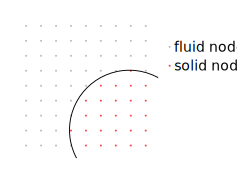
\includegraphics[width=\singleimagewidth]{figures/lbm/dem-to-lbm-mapping.pdf}
	\caption{An example of the mapping process from DEM to LBM structures. Nodes are assigned as fluid or solid based on relative location of pebble centroid and radius. Here we have a resolution of 9 (\textit{i.e.} 9 nodes per pebble diameter).}\label{fig:dem-2-lbm-example1}
\end{figure}
\begin{figure}[ht]
	\centering
	\includegraphics[width=\doubleimagewidth]{figures/lbm/lbm-pebble-res25.png}
	\caption{A three-dimensional DEM pebble as imported into the LBM lattice with a resolution of 25.}\label{fig:dem-2-lbm-example2}
\end{figure}
\begin{figure}[ht]
	\centering
	\includegraphics[width=\doubleimagewidth]{figures/lbm/crossSection0024.jpg}
	\caption{A two-dimensional slice of a DEM pebble bed as imported into the LBM lattice with a resolution of 25.}\label{fig:dem-2-lbm-example3}
\end{figure}
\begin{figure}[ht]
	\centering
	\includegraphics[width=\textwidth]{figures/lbm/palabos_packing_fraction}
	\caption{The digital packing fraction was measured at all slices through the height of the pebble bed. When the average value equaled the expected value, the mapping from DEM to LBM was considered consistent.}\label{fig:dem-2-lbm-packing-fraction}
\end{figure}

In the example of Fig.~\ref{fig:dem-2-lbm-example1}, the resolution is only 9. Thus 9 nodes are needed to span the diameter of a single pebble and the lattice spacing is $\delta_x = 1/9$. In the second example shown in Fig.~\ref{fig:dem-2-lbm-example2}, we see a pebble in three dimensions that has been mapped onto the LBM nodes with a resolution of 25 (thus $\delta_x = 1/25$). The trade-off between a small lattice spacing is in the ability to resolve the spherical surface of the pebble, stability, and even the ability to resolve a proper packing fraction in the pebble bed. 

Shown in Fig.~\ref{fig:dem-2-lbm-example3} is a single slice of a pebble bed with a resolution of 25 as it is mapped into LBM. Here, black pixels represent solid and white pixels are fluid. Because we are representing the surfaces of curved objects with straight lines, at the point of contact between pebbles, the mapping from DEM to LBM would occasionally over-predict the overlap between pebbles. This was measured numerically by comparing the number of white pixels to black pixels in each slice -- the digital equivalent of a packing fraction,
\begin{equation}
	\phi_{d,j} = \frac{N_\text{black}}{N_\text{white}}
\end{equation}

The total digital packing fraction of the ensemble, as mapped into LBM, is simply
\begin{equation}
	\phi_d = \frac{1}{J}\sum_j^J\phi_{d,j}
\end{equation}

where there are $J$ total slices. For example, we see in Fig.~\ref{fig:dem-2-lbm-packing-fraction} a plot of the digital packing fraction moving through the pebble bed. The digital mapping of DEM onto LBM was tweaked with a radius magnification parameter until the digital packing fraction matched the calculated packing fraction from DEM. When the error between digital and continuous packing fractions was small, as calculated by
\begin{equation}
	\Phi_{err} = \frac{|\phi_d - \phi|}{\phi} < 10^{-4}
\end{equation}
I considered the mapping from DEM to LBM to be consistent.
\FloatBarrier


\subsection{Numerical Implementation of LBM and DEM Coupling}\label{sec:lbm-solver}

As usual, the packing structure of our pebble bed is rendered with the code LIGGGHTS. Details of the software are described in \cref{sec:dem-solver}. The DEM solver is a highly parallel C++ code based on the Molecular Dynamics (MD) code LAMMPS.\cite{Plimpton1995} 

The translation between the DEM packing and LBM nodal network is done with Python scripts I created to discretize and digitize the `spherical' information of DEM into LBM.

To solve the lattice-Boltzmann collision and streaming equations, we make use of the open-source code maintained by FlowKit Ltd named Palabos.\cite{Flow} The Palabos library provides an interface for quick implementation of lattice-Boltzmann models in C++. Implemented models include the BGK and thermal flows with the Boussinesq approximation, among many others. The lattices available are the common grids of D2Q9, D3Q13, D3Q15, D3Q19, or D3Q27. Zou/He, periodic, and bounce-back conditions are built into the LB kernel; implementation of Dirichlet or Neumann conditions with velocity or pressure are also available. The software is freely available under the terms of the open-source AGPLv3 license.\cite{FreeSoftwareFoundationInc.2007} All mentioned models and ingredients are parallelized with MPI, including the I/O operations that are implemented in terms of MPI’s Parallel I/O API.




%%%%%%%%%%%%%%%%%%%%%%%%%%%%%%%%%%%%%%%%%%%%%%%%%%%%%%%%%%%%%%%%%%%%%%%%%%%%%%%%%%%%%%%%%%%%%%%%%%%%%%%%%%%%
%%%%%%%%%%%%%%%%%%%%%%%%%%%%%%%%%%%%%%%%%%%%%%%%%%%%%%%%%%%%%%%%%%%%%%%%%%%%%%%%%%%%%%%%%%%%%%%%%%%%%%%%%%%%
%
% new section
%
%%%%%%%%%%%%%%%%%%%%%%%%%%%%%%%%%%%%%%%%%%%%%%%%%%%%%%%%%%%%%%%%%%%%%%%%%%%%%%%%%%%%%%%%%%%%%%%%%%%%%%%%%%%%
%%%%%%%%%%%%%%%%%%%%%%%%%%%%%%%%%%%%%%%%%%%%%%%%%%%%%%%%%%%%%%%%%%%%%%%%%%%%%%%%%%%%%%%%%%%%%%%%%%%%%%%%%%%%
\section{Summary of LBM Modeling Development}


The DEM code covered in this chapter is the foundation upon which the majority of my numeric work rests. The core of the code employed in this dissertation are from open-sourced, crowd-supported, libraries and routines. Along the process of developing the tools and adapting them to the specific needs of the ceramic breeders, I will introduce several new models and algorithms. The enhancements to the code represent a significant contribution to the design tools that will be available to solid breeder designers upon the successful completion of this dissertation.

While concurrently developing the dynamic-coupling tools for the CFD-DEM models, I recognized the potential need for modeling the meandering path of low-$\Re$ flow of helium in our packed bed with heat generation. The sacrifice we make to achieve the numerical fidelity is that in this implementation of fluid-particle interaction there is only a static coupling. The pebble-scale micromechanical interaction information for pebble damage modeling is still solved transiently in the DEM computations. A snapshot of the structure is discretized and loaded into the LBM solver which then calculates temperature and velocity fields of both solid and fluid phases. There is no cross-communication in this technique as the packing structure is effectively frozen during the LBM calculations.

The LBM approach was chosen in place of finite element or finite volume methodology because of issues with discretization of meshes in a three dimensional packed bed with interstitial gas. There are techniques to handle packed beds with continuum fluid mechanics software, but the size of packed beds we are interested in make the FEM approach intractable.

Furthermore, the simple LBM formulation of enforcing no-slip conditions on complex geometry is trivially realized with bounce-back rules on distribution functions. The multi-relaxation-time lattices for momentum and energy offer complete modeling of complex geometry and conjugate heat transfer with far less computational overhead compared to FEM models.